% !TeX source = ../main.tex

\chapter[Introduction]{Introduction}

\section{Notations on Sobolev spaces}
\label{sec:sobolev_notations}

\begin{figure}[!ht]
  \centering
  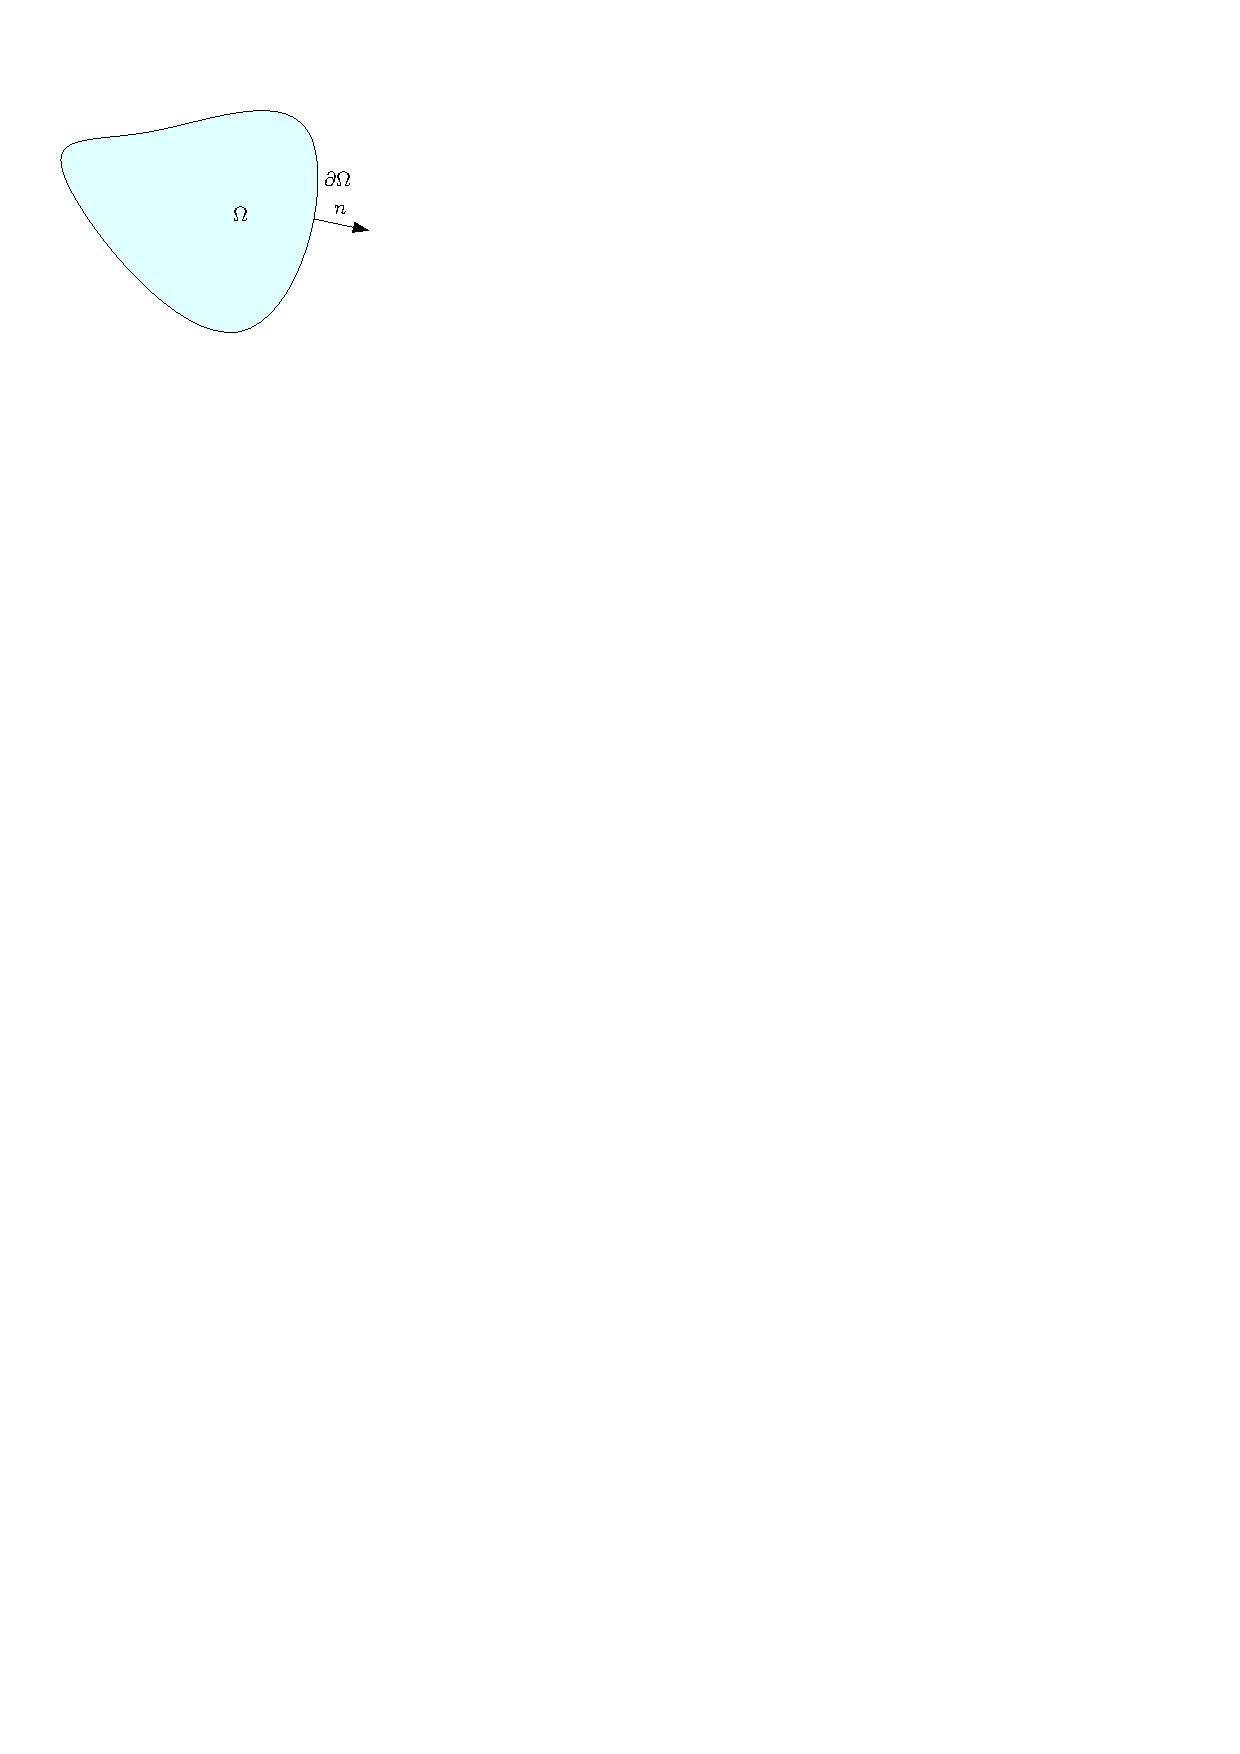
\includegraphics{domain}
  \caption{A Lipschitz domain $\Omega$ and its boundary $\partial\Omega$. We generally indicate with $n$ the outer normal to the boundary.}
  \label{fig:domain}
\end{figure}

Let $\Omega \subset \R^d$ be an open, bounded domain with Lipschitz boundary $\partial\Omega$. We begin by introducing some standard functional spaces that will be used throughout this course.

\subsection{Lebesgue spaces}

For $1 \leq p < \infty$, we define the Lebesgue space $L^p(\Omega)$ as the set of measurable functions $u: \Omega \to \R$ such that
\[
\|u\|_{L^p(\Omega)} := \left(\int_\Omega |u(x)|^p \diff x \right)^{1/p} < \infty.
\]

For $p = \infty$, we define $L^\infty(\Omega)$ as the space of essentially bounded measurable functions with the norm
\[
\|u\|_{L^\infty(\Omega)} := \operatorname{ess\,sup}_{x \in \Omega} |u(x)| < \infty.
\]

Finally we define the space of locally integrable functions as $L^1_{loc}(\Omega)$ where every function $u: \Omega \to \R$ is:
\begin{itemize}
\item measurable;
\item $u|_{K} \in L^1(K)$ for each compact subset $K \subseteq \Omega$.
\end{itemize}

These spaces, equipped with their respective norms, are Banach spaces. In particular, $L^2(\Omega)$ is a Hilbert space with the inner product
\[
(u, v)_{L^2(\Omega)} = \int_\Omega u(x) v(x) \diff x.
\]



\subsection{Weak derivatives}

Let $\alpha = (\alpha_1, \alpha_2, \ldots, \alpha_d)$ be a multi-index with $|\alpha| = \alpha_1 + \alpha_2 + \cdots + \alpha_d$. For a function $u \in C^{|\alpha|}(\Omega)$, we define the standard partial derivative
\[
D^\alpha u = \frac{\partial^{|\alpha|} u}{\partial x_1^{\alpha_1} \partial x_2^{\alpha_2} \cdots \partial x_d^{\alpha_d}}.
\]

For functions that are not sufficiently smooth, we introduce the concept of weak derivatives.

\begin{definition}[Weak derivative]
Let $u \in L^1_{\text{loc}}(\Omega)$ and $\alpha$ be a multi-index. A function $v \in L^1_{\text{loc}}(\Omega)$ is called the $\alpha$-th weak derivative of $u$, denoted by $D^\alpha u = v$, if
\[
  \int_\Omega v(x) \phi(x) \diff x =  (-1)^{|\alpha|} \int_\Omega u(x) D^\alpha \phi(x) \diff x  \quad \forall \phi \in C_0^\infty(\Omega).
\]
\end{definition}

\subsection{Sobolev spaces $W^{k,p}(\Omega)$ and $H^k(\Omega)$}

For integers $k \geq 0$ and $1 \leq p \leq \infty$, we define the Sobolev space $W^{k,p}(\Omega)$ as
\[
W^{k,p}(\Omega) = \{u \in L^p(\Omega) : D^\alpha u \in L^p(\Omega) \text{ for all } |\alpha| \leq k\},
\]
where $D^\alpha u$ are weak derivatives. For $p < \infty$, this space is equipped with the norm
\[
\|u\|_{k,p,\Omega} := \left( \sum_{|\alpha| \leq k} \|D^\alpha u\|_{L^p(\Omega)}^p \right)^{1/p}.
\]

For $p = \infty$, we define
\[
\|u\|_{k,\infty,\Omega} = \max_{|\alpha| \leq k} \|D^\alpha u\|_{L^\infty(\Omega)}.
\]

We also define the seminorm
\[
|u|_{k,p,\Omega} = \left( \sum_{|\alpha| = k} \|D^\alpha u\|_{L^p(\Omega)}^p \right)^{1/p},
\]
with a similar modification for $p = \infty$.

When $p = 2$, we denote $W^{k,2}(\Omega)$ by $H^k(\Omega)$, which is a Hilbert space with the inner product
\[
(u, v)_{H^k(\Omega)} = \sum_{|\alpha| \leq k} (D^\alpha u, D^\alpha v)_{L^2(\Omega)}.
\]

In this case, we simplify the notation for the definition of the norm, and we omit the subscript $2$ (and the domain $\Omega$ if no confusion can arise) for the $H^k$-norm:
\[
  \|u\|_{k} \equiv \|u\|_{k,\Omega} := \|u\|_{k,2,\Omega} = \left( \sum_{|\alpha| \leq k} \|D^\alpha u\|_{L^2}^2 \right)^{1/2}.
\]

\subsection{Sobolev spaces with vanishing boundary values}

For functions in Sobolev spaces, we define the subspace of functions vanishing on the boundary $\partial\Omega$. For $1 \leq p < \infty$, we define
\[
W_0^{k,p}(\Omega) = \overline{C_0^\infty(\Omega)}^{\|\cdot\|_{W^{k,p}(\Omega)}},
\]
that is, the closure of $C_0^\infty(\Omega)$ with respect to the $W^{k,p}$-norm.

In particular, we denote $W_0^{k,2}(\Omega)$ by $H_0^k(\Omega)$. A key property of $H_0^1(\Omega)$ is the Poincaré inequality, which states that there exists a constant $C_{\Omega} > 0$ such that
\[
\|u\|_{L^2(\Omega)} \leq C_{\Omega} \|\nabla u\|_{L^2(\Omega)} \quad \forall u \in H_0^1(\Omega).
\]

This implies that the seminorm $|u|_{H^1(\Omega)} = \|\nabla u\|_{L^2(\Omega)}$ is actually a norm on $H_0^1(\Omega)$ equivalent to the standard $H^1$-norm.

\subsection{Dual spaces}

For a Banach space $X$, we denote by $X'$ its dual space, i.e., the space of continuous linear functionals on $X$. For example, $H^{-1}(\Omega) = (H_0^1(\Omega))'$ denotes the dual of $H_0^1(\Omega)$. We indicate with $\langle \cdot, \cdot \rangle$ the duality pairing between $X$ and $X'$, and we write $f(u) \equiv \langle f, u \rangle$ for $f \in X'$ and $u \in X$.

The norm of a functional $f \in X'$ is defined as
\[
\|f\|_{X'} = \sup_{u \in X} \frac{|\langle f, u \rangle|}{\|u\|_X}.
\]

\subsection{Riesz representation theorem}

For Hilbert spaces, we have a powerful characterization of the dual space through the Riesz representation theorem.

\begin{theorem}[Riesz representation theorem]
  \label{theo:riesz_representation}
Let $H$ be a Hilbert space with inner product $(\cdot, \cdot)_H$. For every bounded linear functional $f \in H'$, there exists a unique element $\tau f \in H$ such that
\[
f(v) = \langle f, v \rangle = (\tau f, v)_H \quad \forall v \in H,
\]
and furthermore,
\[
\|f\|_{H'} = \|\tau f\|_H.
\]
The operator $\tau$ is the so called Riesz operator.
\end{theorem}

This theorem establishes an isometric isomorphism between a Hilbert space and its dual. In particular, for $H = L^2(\Omega)$, given $f \in L^2(\Omega)$, we can identify the functional 
\[
v \mapsto \int_\Omega f v \, \mathrm{d}x
\]
with $f$ itself. Similarly, for $H = H^1_0(\Omega)$, every element in $H'$ can be represented uniquely as an inner product with some element in $H$.

The Riesz representation theorem is especially useful in characterizing the action of operators and in proving existence of solutions to variational problems, as it allows us to convert abstract duality pairings into concrete inner products.

\subsection{Bilinear forms and operators}

Let $X$ and $Y$ be Banach spaces. A bilinear form $a: X \times Y \to \mathbb{R}$ is said to be bounded (or continuous) if there exists a constant $C > 0$ such that
\[
|a(u, v)| \leq C \|u\|_X \|v\|_Y \quad \forall u \in X, \forall v \in Y.
\]

Given a bilinear form $a: X \times Y \to \mathbb{R}$, we can define its associated operator $A: X \to Y'$ by
\[
\langle Au, v \rangle = a(u, v) \quad \forall u \in X, \forall v \in Y,
\]
where $\langle \cdot, \cdot \rangle$ denotes the duality pairing between $Y'$ and $Y$.

The operator $A$ is linear and it inherits the boundedness of $a$, i.e.,
\[ 
  \|A\|_* := \|A\|_{\mathcal{L}(X,Y')} = \sup\limits_{u \in X, v \in Y} \frac{|a(u,v)|}{\|u\|_X \|v\|_Y}.
\]

When $X = Y$ is a Hilbert space, a bilinear form $a: X \times X \to \mathbb{R}$ is said to be:
\begin{itemize}
  \item Symmetric if $a(u, v) = a(v, u)$ for all $u, v \in X$
  \item Coercive (or elliptic) if there exists $\alpha > 0$ such that $a(u, u) \geq \alpha \|u\|_X^2$ for all $u \in X$
\end{itemize}

\subsection{Trace spaces and the trace operator}
\rev{L'operatore traccia viene introdotto formalmente nella sezione \ref{sec:trace_operators}, spostarlo qui forse?}


For functions in $H^1(\Omega),$ we can define their traces on the boundary $\partial\Omega$. The trace operator 
\[
\gamma: H^1(\Omega) \to H^{1/2}(\partial\Omega)
\]
is a bounded linear operator that extends the classical restriction to the boundary. For simplicity, we often write $u|_{\partial\Omega}$ for $\gamma(u)$.

The space $H^{1/2}(\partial\Omega)$ is a fractional Sobolev space on the boundary, and it can be characterized as the set of traces of $H^1(\Omega)$ functions.

A fundamental result is that $u \in H_0^1(\Omega)$ if and only if $u \in H^1(\Omega)$ and $\gamma(u) = 0$.

\subsection{Sobolev embeddings}

Sobolev spaces embed into other spaces in ways that formalize the intuitive notion that functions with more derivatives tend to be more regular. The Sobolev embedding theorems are crucial tools that allow us to relate Sobolev spaces to classical function spaces.

\begin{theorem}[Sobolev embedding]
Let $\Omega \subset \mathbb{R}^d$ be a bounded domain with Lipschitz boundary, $k \geq 0$ an integer, and $1 \leq p < \infty$. Then:

\begin{enumerate}
  \item If $kp > d$, then the following continuous embedding holds:
  \[
  W^{k,p}(\Omega) \hookrightarrow C^{0}(\overline{\Omega}),
  \]
  i.e., every function in $W^{k,p}(\Omega)$ has a continuous representative.
  
  \item If $s \geq 1$, $p,q \in [1, \infty]$, and 
  \[
  s - \frac{d}{p} > k - \frac{d}{q},
  \]
  then the following continous inclusion holds true:
  \[ 
    W^{s,p}(\Omega) \subset W^{t,q}(\Omega).
  \]
\end{enumerate}
\end{theorem}

The first case is of particular interest when we need our functions to be continuous. The condition $kp > d$ gives us a relationship between:

\begin{itemize}
  \item The order of derivatives $k$
  \item The integrability $p$ of those derivatives
  \item The dimension $d$ of the domain
\end{itemize}

For example, in two dimensions ($d=2$):
\begin{itemize}
  \item $H^2(\Omega) = W^{2,2}(\Omega) \hookrightarrow C^0(\overline{\Omega})$ since $2 \cdot 2 > 2$
  \item $W^{1,p}(\Omega) \hookrightarrow C^0(\overline{\Omega})$ for any $p > 2$
  \item $H^{1}(\Omega) \not\hookrightarrow C^0(\overline{\Omega})$.
\end{itemize}

More generally, in $d$ dimensions, we need $k > \frac{d}{p}$ to ensure continuity.

These embedding results are particularly important in numerical analysis, as they help determine when finite element approximations lead to continuous functions. For standard Lagrangian finite elements, the continuity of basis functions is essential, and these embedding theorems provide the theoretical foundation for when such continuity can be expected.

%****************************************************************
% Lezione 27 febbraio
%****************************************************************

\section{Model problem: the Poisson equation}

\subsection{Strong formulation}
Let $\Omega$ be an open, bounded, Lipschitz subset of $\R^d$. Let also $\partial\Omega$ be its boundary.
Consider the following Poisson problem:
\[
\begin{cases} \marginpar{Strong formulation of Poisson problem}
-\Delta u = f \qquad &\text{in $\Omega$} \\
u =  0 \qquad &\text{on $\partial \Omega$}
\end{cases}
\]
where, as usual,
\[
\Delta = \sum_{i=1}^d \frac{\partial^2}{\partial x_i^2}.
\]
If we want to find a numerical solution for this problem, two approaches can be followed:
\begin{itemize}
\item discretize $-\Delta$ (\emph{finite differences});
\item consider the \emph{weak formulation} of the problem (\emph{finite elements}).
\end{itemize}

Finite differences work well if $\Omega$ is a rectangular or parallelepiped domain (e.g. a square, a cube and so on) and if $f$ is regular enough (e.g. continuous). In applications, however, the domain's boundary may not be nice at all, and $f$ may not even be continuous.
The finite element approach tries to overcome these difficulties, by shifting the problem to finding a good finite dimensional space that approximates the functional space where the exact solution lives.

The advantage, when compared to, e.g., finite differences, is that we don't discretize the differential operator -- which maintains its (weak) continuous definition --  but instead we restrict our exploration of candidate solutions to simpler spaces (i.e., spaces of piecewise polynomial functions), for which we can easily compute the action of the differential operator in an exact way.

\subsection{Weak formulation}
To make a concrete example, let us consider the Poisson problem, and let's derive its weak formulation.
Let $\phi \in \D$ a test function (usually $\D=C_0^\infty(\Omega)$). We multiply by $\phi$ both sides of the PDE in the strong formulation and then integrate:
\[
\int_\Omega -\Delta u \phi = \int_\Omega f \phi.
\]
If we integrate by parts and use the fact that $\restr{u}{\partial \Omega} = \restr{\phi}{\partial\Omega} = 0$, we get:
\[
\int_\Omega \nabla u \nabla \phi = \int_\Omega f \phi.
\]
In general we replace $\D$ with a Sobolev space $V$ such that every entry of the weak formulation makes sense. In this case, the weak formulation will be: given $f\in V'$, find $u\in V$ such that
\begin{equation} \label{eqn:weak_1} \marginpar{Weak form (1)}
\int_\Omega \nabla u \nabla v = \int_\Omega f v \quad \forall v\in V.
\end{equation}
with the agreement that, being $f \in V'$, the RHS is in fact a duality.

On one side, we need that $\int_\Omega | \nabla u \nabla v | < +\infty$, and on the other side, we need that $u$ and $v$ should be zero on the domain boundary. For the example above, the natural choice is then the Hilbert space $H^1_0(\Omega)$.

\subsection{Lax-Milgram lemma}
How do we guarantee that a solution to such problem exists? We prove this in an abstract Hilbert setting:
\begin{lemma}[Lax-Milgram]\label{lemma:lax-milgram}\marginpar{Lax-Milgram lemma}
Let $V$ be a Hilbert space and let $a: V\times V \to \R$ be a bilinear operator such that:
\begin{itemize}
\item $a$ is \emph{bounded}, i.e. $\exists c>0$ s.t. 
\[
 a(u,v) \le c \norm{u}_V \norm{v}_V \qquad \forall u,v \in V;
 \]
\item $a$ is \emph{coercive}, i.e. $\exists \alpha >0$ s.t.
\[
  a(u,u) \ge \alpha \norm{u}_V^2 \qquad \forall u \in V.
\]
\end{itemize}
Then, given $f\in V'$, the following problem
\begin{equation}\label{eqn:weak_laxmilgram}
a(u,v) = \langle f,v \rangle \quad \forall v\in V
\end{equation}
admits a unique solution $u$. Moreover, $u$ satisfies the following inequality:
\[
\norm{u}_V \le \frac{\norm{f}_{V'}}{\alpha}.
\]
\end{lemma}
\begin{proof}
  Let's consider the linear operator $A: V \to V'$ defined by $A(u) = a(u,\cdot)$.
  Boundedness of $a$ implies that $A$ is a bounded operator, and coercivity implies that 
  \[
    \langle A u, u \rangle = a(u,u) \ge \alpha \norm{u}_V^2 \quad \forall u \in V.
  \]
  
  Let us consider the map $\phi: V \mapsto V$ defined by 
  \[ 
    \phi(v) = v - \rho \tau(A v - f),
  \]
  where $\rho$ is a positive constant to be chosen later, and $\tau$ is the Riesz operator defined in Theorem~\ref{theo:riesz_representation}. By construction, if $u$ is a fixed point of $\phi$, i.e., $u= \phi(u)$, then $u$ necessarily satisfies $A u = f$. Conversely, if $u$ satisfies $Au=f$, then $u$ is also a fixed point of $\phi(u)=u$. 
  
  We want to show that ellipticity is enough to guarantee that there exists a $\rho$ such that $\phi$ is a contraction, i.e., $\exists! ~u$ s.t. $Au=f$.
  
  We have:
  \begin{align*}
    \norm{\phi(u) - \phi(v)}_V^2 & = \norm{u - v - \rho \tau(A(u - v))}_V^2 \\
    & = \norm{u - v}_V^2 - 2 \rho \langle A(u - v), u - v \rangle + \rho^2 \norm{A(u - v)}_{V'}^2 \\
    & \leq \norm{u - v}_V^2 - 2 \rho \alpha \norm{u - v}^2_V + \rho^2 \|A\|^2 \norm{u - v}_V^2 \\
    & \leq  (1 - 2\rho \alpha + \rho^2 \|A\|^2) \norm{u - v}_V^2.
  \end{align*}
  By choosing $\rho$ such that $0<1 - 2\rho \alpha + \rho^2 \|A\|^2 < 1$, (i.e., $\rho<\frac{2\alpha}{\|A\|}$) we have that $\phi$ is a contraction, and by the Banach fixed point theorem, we have that there exists a unique fixed point $u$ of $\phi$, which is the solution of the problem.
  
  Finally, we can estimate the norm of $u$ by the norm of $f$ and the coercivity constant $\alpha$:
  \[
  \alpha \norm{u}_V^2 \leq \langle A u, u \rangle = \langle f, u \rangle \leq \norm{f}_{V'} \norm{u}_V \qquad \Longrightarrow \qquad \norm{u}_V \leq \frac{\norm{f}_{V'}}{\alpha}.
  \]
\end{proof}

In the Poisson problem's case, the bilinear operator is
\[
a(u,v) = \int_\Omega \nabla u \nabla v,
\]
which is clearly bounded and coercive if $V=H_0^1(\Omega)$. In particular, coercivity follows from Poincaré inequality which implies that the norm in $H^1(\Omega)$ is equivalent to the $H^1$ seminorm when the solution is zero on the boundary:
\[
c_1 \norm{u}_{1} \leq \abs{u}_{1,2} = \norm{\nabla u}_{L^2} \leq c_2 \norm{u}_{1} \qquad \forall u \in H_0^1(\Omega).
\]
Hence, the weak formulation of the Poisson problem admits a unique solution by Lax-Milgram lemma.

\subsection{Functional minimization}

\begin{theorem}[Minimization problem]
When the bilinear operator $a$ is also symmetric (i.e., $a(u,v) = a(v,u)$ for any pair $u,v \in V$), then existence and uniqueness of a solution to the weak formulation~\eqref{eqn:weak_1} is equivalent to finding the unique minimizer of the quadratic (and strongly convex) minimization problem:
\[
u = \arg\min_{v \in V} \Phi(v) := \frac{1}{2} a(v,v) - \langle f, v \rangle.
\]
\end{theorem}
\begin{proof}
 We start by showing that if $u$ is a minimizer of $\Phi$, then it satisfies the weak formulation. We have in fact that for any $v$ in $V$, and for any $\varepsilon \in \R^+$:
 \begin{equation*}
\begin{split}
  \Phi(u) \leq \Phi(u+\varepsilon v)  & = \frac{1}{2} a(u+\varepsilon v, u+\varepsilon v) - \langle f, u+\varepsilon v \rangle \\
  & = \Phi(u) + \varepsilon a(u,v) + \frac{\varepsilon^2}{2} a(v,v) - \varepsilon \langle f, v \rangle, \\
  - \frac{\varepsilon^2}{2} \alpha \|v\|^2 \leq - \frac{\varepsilon^2}{2} a(v,v) & \leq \varepsilon a(u,v) - \varepsilon \langle f, v \rangle \\
  - \frac{\varepsilon}{2} \alpha \|v\|^2 & \leq a(u,v) - \langle f, v \rangle \leq \frac{\varepsilon}{2} \alpha \|v\|^2,
  \end{split}
 \end{equation*}
 where the second line follows by the symmetry of the bilinear form $a$, while the last chain of inequalities follow from dividing once for $\varepsilon$, and once for $-\varepsilon$ both sides of the inequality. We can now take the limit $\varepsilon \to 0$ and we get that
  \[
  a(u,v) = \langle f, v \rangle \quad \forall v \in V.
  \]
  Conversely, if $u$ satisfies the weak formulation, we can show that it is a minimizer of $\Phi$.
  We have:
  \[
  \begin{split}
  \Phi(v) - \Phi(u) & = \frac{1}{2} a(v,v)  \underbrace{- \langle f, v \rangle}_{= - a(u,v)=-\frac12a(u,v)-\frac12a(v,u)} - \frac{1}{2} a(u,u)  + \underbrace{\langle f, u \rangle}_{=a(u,u)} \\
   & = \frac{1}{2} a(v-u,v-u) \geq \frac{\alpha}{2} \|v-u\|_V^2, 
  \end{split}
  \]
  where we used the coercivity of $a$ and the symmetry of $a$ to rearrange the terms. This shows that $\Phi(u)$ is a global minimum of $\Phi$, and since $\Phi$ is strongly convex, it is also the unique minimizer.
\end{proof}

\subsection{Ceà's lemma}
Lax-Milgram lemma guarantees the existence of a unique solution to the weak
problem, but it does not provide any information about the error we make when we
restrict our search to a finite dimensional space. 

One of the reason why the finite element method is powerful is that the
differential operators stay untouched and, instead, what is to be simplified is
\emph{the set in which the solutions live}. This fact makes it possible to
derive a very simple yet powerful property of the finite element approximations,
namely, the \emph{orthogonality property of the error}. We construct a sequence
of subspaces $V_h \subset V$ such that $V_h = \Span\{v_i\}_{i=1}^n$, with $n$
depending on $h$. Then we restrict the weak problem to $V_h$, which inherits the
norm from $V$: given $f \in V'$, find $u_h \in V_h$ s.t.
\begin{equation} \label{eqn:weak_2} \marginpar{Discrete weak form}
a(u_h,v_h) = \langle f,v_h \rangle \quad \forall v_h\in V_h.
\end{equation}
The element $u_h$ will be our candidate approximate solution. Since $V_h$ is a Hilbert space, and the bilinear operator $a(\cdot, \cdot)$ is coercive in the entire $V$, then also Problem~\eqref{eqn:weak_2} satisfies the hypotheses of Lax-Milgram lemma, and we conclude that there exists a unique solution. For completeness, however, we shall  prove its existence also using Ritz method.

Since $u_h \in V_h$, there exist a unique set of coefficients $\{u^j\}_{j=1}^n$ such that
\[
u_h = \sum_{j} u^j v_j.
\]
The discrete counterpart of the weak problem \ref{eqn:weak_2} then becomes:
\[
a\left(\sum_{j} u^j v_j ,v_h\right) = \langle f,v_h \rangle \quad \forall v_h\in V_h.
\]
In particular, it will suffice for us to check it for a basis of $V_h$:
\[
\sum_{j} a(v_j, v_i)  u^j = \langle v_i,f \rangle \quad \forall i=1,\dots,n.
\]
Here we have rearranged the objects in the brackets and used linearity to make it clearer that this is a matrix identity: if $A$ is the matrix whose entries are $A_{ij}=a(v_j, v_i)$, then we have to solve the linear system
\[
A \mathbf{u} = \mathbf{f}
\]
where $\mathbf{u}=\{u^i\}_{i=1}^n$ and $\mathbf{f}=\{\langle f, v_i\rangle\}_{i=1}^n$.
In particular, $A$ is clearly symmetric and positive definite due to the coercivity of $a$:
\[
\mathbf{u}^T A \mathbf{u} = a(\sum_{i} u^i v_i, \sum_{j} u^j v_j) \ge \alpha \norm{\sum_{i} u^i v_i}^2 \ge 0
\]
and this, by linearity, is zero if and only if every $u^i$ is zero. We conclude that $A$ is non singular, hence $u_h$ exists and is unique.

We now seek a way to control \emph{a priori} the error introduced by the restriction to $V_h$.
\begin{lemma}[Ceà]\marginpar{Ceà's lemma} \label{lemma:cea}
In the setting of Lax-Milgram lemma, let $u\in V$ be the solution of the weak problem~\eqref{eqn:weak_laxmilgram} and $u_h \in V_h$ a solution of~\eqref{eqn:weak_2}. Then:
\[
\norm{u - u_h} \le \frac{\norm{A}}{\alpha} \inf_{v_h \in V_h} \norm{u - v_h}.
\]
\end{lemma}
\begin{proof}
Observe that, since $u$ solves the weak problem in the whole $V$, then also
\[
a(u,v_h) = \langle f,v_h \rangle \quad \forall v_h\in V_h.
\]
By linearity, it follows that
\[
a(u - u_h,v_h) = 0 \quad \forall v_h\in V_h.
\]
In particular, this is also true if we substitute $v_h$ with $v_h - u_h$, which is still in $V_h$:
\[
a(u - u_h, v_h - u_h) = 0 \quad \forall v_h\in V_h.
\]
This is an orthogonality property of the error. Now we exploit the properties of $a$:
\begin{align}
\alpha \norm{u - u_h}^2 & \le a(u - u_h, u - u_h) \\
& = a(u - u_h, u - v_h) + a(u - u_h, v_h - u_h) \\
& = a(u - u_h, u - v_h) \\
& \le \norm{A} ~\norm {u - u_h} ~ \norm {u - v_h} \quad \forall v_h \in V_h.
\end{align}
The thesis follows by simplifying $\norm{u - u_h}$ on both sides of the inequality, and taking the infimum over $v_h \in V_h$.
\end{proof}

The lemma shows that the error in the finite element approximation is proportional to the best possible approximation in $V_h$, i.e., the error is controlled by the distance between the exact solution $u$ and the finite dimensional space $V_h$. This will be exploited in the next sections to derive both \emph{a-priori} and \emph{a-posteriori} error estimates for the finite element method.

\subsection{The one-dimensional case}

Let $\Omega = (a,b)$. We consider a set of $n+2$ points $\Set{x_i}_{i=0}^{n+1}$ such that
\[
a = x_0 < x_1 < \dots < x_{n+1} = b.
\]
To keep things simple, let
\[
x_i = a+ih, \quad h = \frac{b-a}{n+1}.
\]
Let $V=H_0^1((a,b))$. Now consider
\[
V_h = \Set{v \in C^0([a,b]): \restr{v}{[x_i, x_{i+1}]}\in \P^1([x_i, x_{i+1}]) \,\forall i=0,\dots,n, \, v(a)=v(b)=0}
\]
where $\P^1$ denotes the space of polynomials of degree at most 1. This space has dimension $n$ and contains piecewise linear functions on $[a,b]$ which are zero on the boundary.

We proceed to find a basis for it: let $v^i(u) := u(x_i)$ the evaluation of $u$ in the node $x_i$, for $i=1,\dots,n$. If $u$ were in $\D$, then $v^i$ would act as a Dirac delta $\delta(x-x_i)$, since
\[
\langle v^i, u \rangle = \int_\Omega \delta(x-x_i) u(x) \diff x = u(x_i).
\]
\begin{figure}[!htb]
\centering
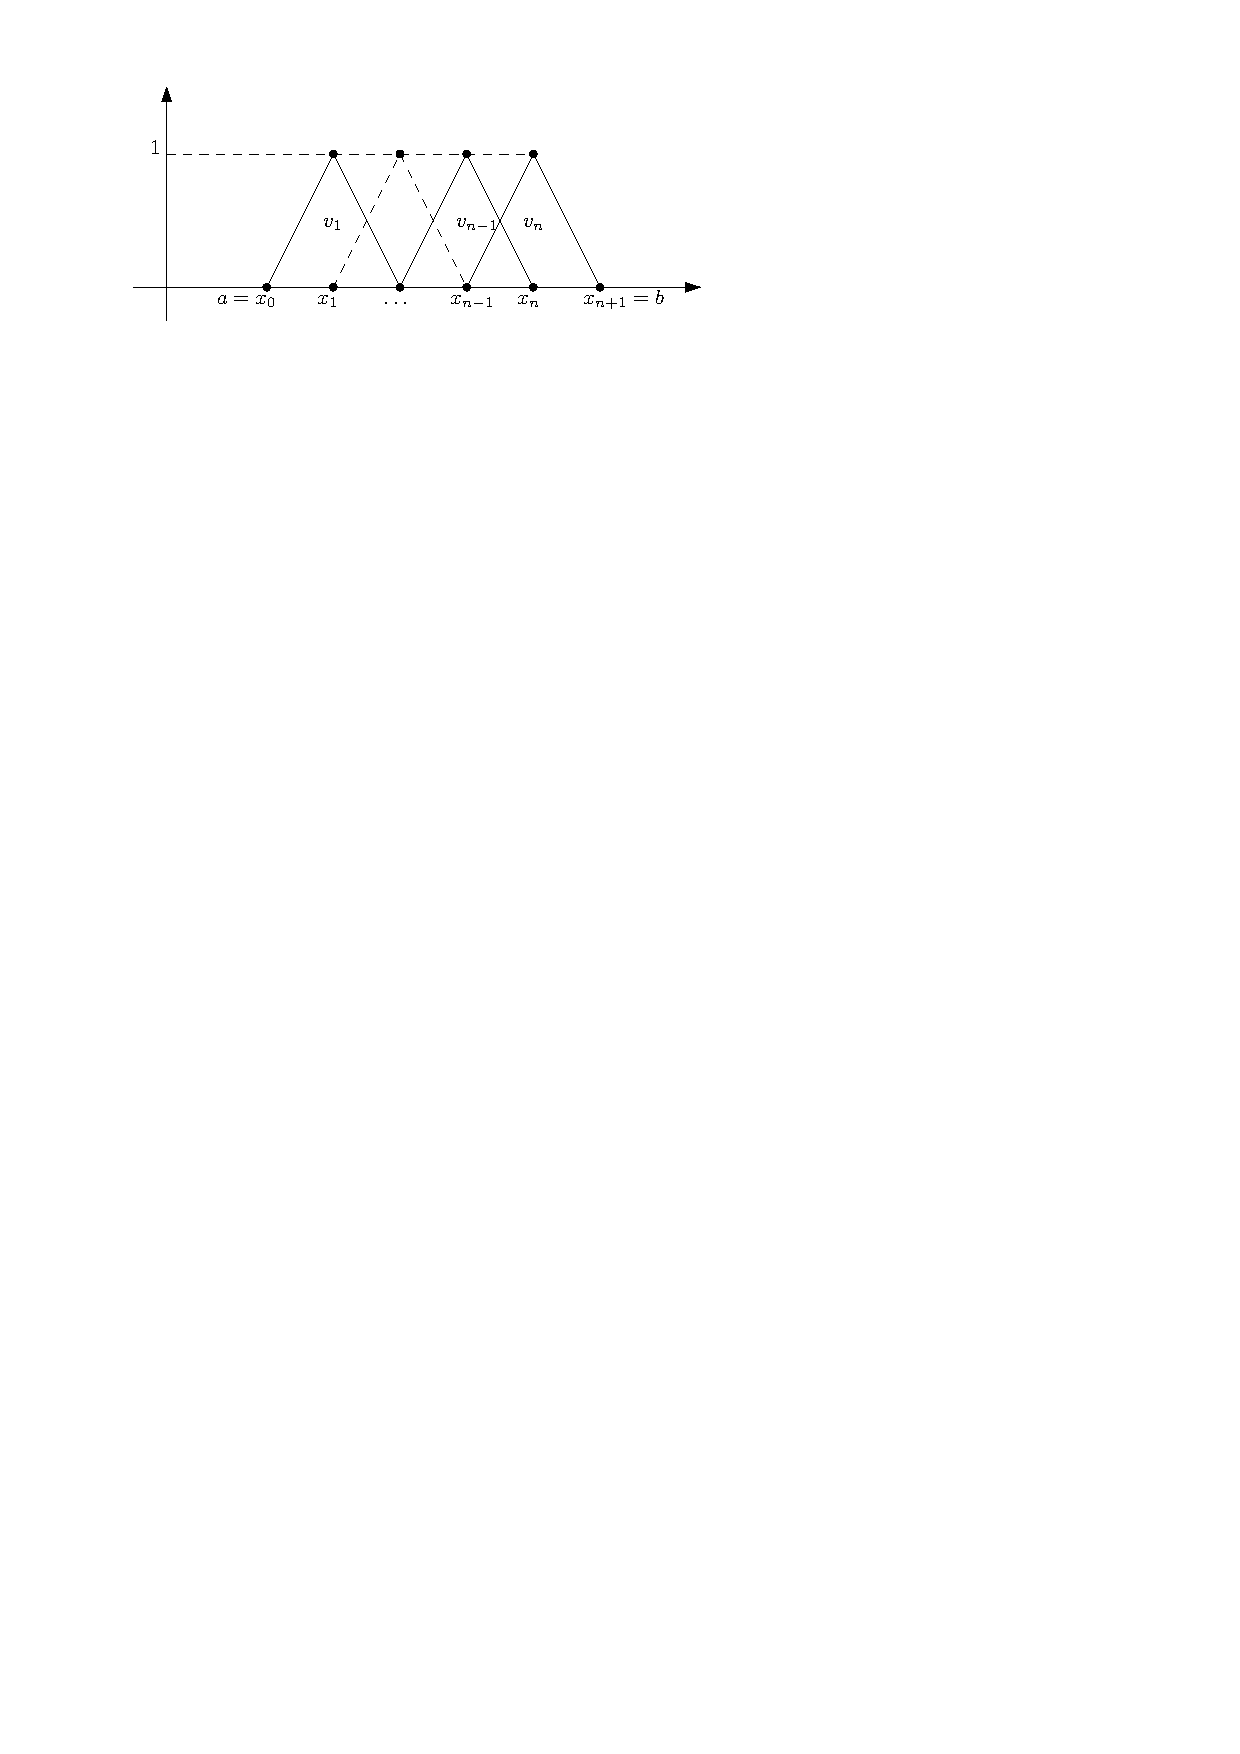
\includegraphics{p1_basis_1d.pdf}
\caption{The basis functions $v_i$ in the 1D case.}
\label{fig:1d_basis}
\end{figure}
We construct functions $v_j \in V_h$ such that
\[
v^i(v_j) = \delta_{ij} = \begin{cases}
1 \quad \text{if } i=j \\
0 \quad \text{if } i\ne j
\end{cases}
\quad \forall i,j \in \{1,\dots,n\}.
\]
For every node $x_j$ in the interior of $[a,b]$ we are considering a piecewise linear function that is one on that node and zero on any other node. It is clear that the functions $\{v_j\}_{j=1}^{n}$\footnote{These functions are also called "Hat functions" for their peculiar hat form.} form a basis for the space $V_h$. These are the so-called \emph{shape functions}. Instead, the $v^i$-s form a basis for $V_h'$ and are called the \emph{nodal basis functions}. The coefficients $\{u^i\}_{i=1}^n\in \R$ such that $u_h = \sum_{i=1}^{n} u^i v_i$ are the \emph{degrees of freedom} (DoFs) of the finite element function $u_h$. 

In the one-dimensional case, the entries of the matrix $A$ are of the form
\[
A_{ij} = \int_a^b v_j'(x) v_i'(x) \diff x.
\]
Since the basis functions have a compact support, it is immediate to notice that $A_{ij} = 0$ whenever the supports of the involved basis functions do not intersect. This is a distinguishing feature of a finite element method: the matrix $A$ is constructed in a way that makes it \emph{sparse}. In particular, in this case we have
\[
A_{ij} = \begin{cases}
0 \quad &\text{if } \abs{i-j}>1 \\
-\frac{1}{h} \quad &\text{if } \abs{i-j}=1 \\
\frac{2}{h} \quad &\text{if } i=j
\end{cases}.
\]
Notice that we have obtained the same matrix we would get with a finite difference method of the same order (with the exception of a scaling factor of $1/h$).

In fact, for a finite difference method, the second derivative approximation using a three-point stencil is given by
\[
-\frac{d^2 u}{dx^2}(x_i) \approx -\frac{u(x_{i-1}) - 2u(x_i) + u(x_{i+1})}{h^2}.
\]

When applied at each interior point of the domain, this leads to the linear system
\[
\frac{1}{h^2}
\begin{bmatrix}
2 & -1 & 0 & \cdots & 0 \\
-1 & 2 & -1 & \cdots & 0 \\
0 & -1 & 2 & \cdots & 0 \\
\vdots & \vdots & \vdots & \ddots & \vdots \\
0 & 0 & 0 & \cdots & 2
\end{bmatrix}
\begin{bmatrix}
u_1 \\
u_2 \\
\vdots \\
u_n
\end{bmatrix}
=
\begin{bmatrix}
f_1 \\
f_2 \\
\vdots \\
f_n
\end{bmatrix}
\]

where $u_i = u(x_i)$ and $f_i = f(x_i)$. The corresponding finite difference matrix can be expressed as:

\[
A_{FD,ij} = \begin{cases}
0 \quad &\text{if } \abs{i-j}>1 \\
-\frac{1}{h^2} \quad &\text{if } \abs{i-j}=1 \\
\frac{2}{h^2} \quad &\text{if } i=j
\end{cases}.
\]

Comparing with the finite element matrix above, we notice that $A_{FD} = -\frac{1}{h} A_{FE}$, meaning they differ only by a constant factor. 

However, there is an important difference in the right-hand sides. In the finite difference method, the right-hand side consists of point evaluations $f_i = f(x_i)$, while in the finite element method, the right-hand side involves integrals $\int_\Omega f v_i \diff x$. For non-smooth functions $f$, these two approaches can yield significantly different results, with the finite element method generally providing better stability for irregular data.

\section{Finite dimensional spaces}

One of the key aspects of the finite element method is the construction of
finite dimensional spaces that approximate infinite dimensional Sobolev spaces,
with good approximation properties. Independently of how we construct such
finite dimensional spaces, we can exploit the fact all such spaces are
iso-morphic to $\R^n$ for some $n$. This in turns implies that any bilinear form
defined on such spaces can be represented as a matrix, and linear functionals
defined on such spaces can be represented as (co-)vectors, opening up the
possibility to use the machinery of linear algebra to solve the resulting
(non-)linear systems.

Let $V$ be a Banach space on the domain $\Omega$, and let $V_h$ be an $h$-parameter family of finite dimensional discretizations of $V$ with finite dimension $n$. We say that $V_h$ is a conforming discretization of $V$, if, for any $h\in \R$, the space $V_h$ is a proper linear subspace of $V$, i.e., $V_h \subseteq V$. 

\subsection{Basis functions}

Generally speaking, we indicate with the set $\{v_i\}_{i=1}^n$ a choice of (linearly independent) basis functions for $V_h$, i.e., 
\[
V_h = \Span\{v_i\}_{i=1}^n, \qquad \forall u_h \in V_h , \quad \exists! \quad \{u^i\}_{i=1}^n \text{ s.t. } u_h(x) = \sum_{i=1}^n u^i v_i(x),
\]
The functions $v_i$ are often also called \emph{shape functions}, and the coefficients $\{u^i\}_{i=1}^n$ are called \emph{degrees of freedom} (DoFs).

\subsection{Nodal functions}

We denote with $V_h'$ the dual space of $V_h$, i.e., the space of continuous linear functionals on $V_h$. Since $V_h$ is finite dimensional, so is $V_h'$, and its dimension is the same of $V_h$. We identify a canonical basis for the dual space $V_h'$ given by a set of $n$ linear functionals on $V_h$, given by $\{v^i\}_{i=1}^n$ such that 
\[
V_h' = \Span\{v^i\}_{i=1}^n, \qquad \forall f_h \in V_h', \quad \exists! \quad \{f_i\}_{i=1}^n \text{ s.t. } f_h(x) = \sum_{i=1}^n f_i v^i(x).
\]

The elements of the canonical basis also called \emph{nodal functions} and are
denoted by $\{v^i\}_{i=1}^n$. A generic element of $V_h'$ is often called a
\emph{co-vector}. The basis (or \emph{shape functions}) and the dual basis (or
\emph{nodal functions}) are related by the following property:
\[
v^i(v_j) = \delta_{ij} = \begin{cases}
1 \quad &\text{if } i=j \\
0 \quad &\text{if } i\ne j
\end{cases}
\quad \forall i,j \in \{1,\dots,n\}.
\]

\subsection{Projection operators}

The functions $v^i$ are linear functionals on $V_h$. By the Hann-Banach extension theorem, we can extend them to functionals in $V'$. We choose $n$ such extensions and call them $\{\tilde{v}^i\}_{i=1}^n$. They are chosen such that
\[
\tilde{v}^i \in V', \qquad \tilde{v}^i(u_h) = v^i(u_h) \quad \forall u_h \in V_h.
\]

With this choice of extensions, we can define a projection operator $\Pi: V \to V_h$ as
\[
\Pi(u) = \sum_{i=1}^n \tilde{v}^i(u) v_i = \sum_{i=1}^n \duality{\tilde{v}^i, u} v_i, 
\]
where $\tilde{v}^i(u)=\duality{\tilde{v}^i, u}$ is the value of the functional $\tilde{v}^i$ applied on the function $u$, and it represents the $i$-th component (or the $i$-th \emph{degree of freedom}) of the function $\Pi(u)$ in the basis $\{v_i\}_{i=1}^n$. The projection operator $\Pi$ maps any function $u \in V$ to its finite dimensional approximation in $V_h$. 

In particular, $\Pi$ is indeed a projection, since for any $u_h\in V_h$, we have 
\[
\begin{split}
  \Pi(u_h) = & \sum_{i=1}^n \tilde{v}^i(u_h) v_i = \sum_{i=1}^n v^i(u_h) v_i = \\
  &\sum_{i=1}^n v^i\left(\sum_{j=1}^n u^j v_j\right) v_i = \sum_{i=1}^n \sum_{j=1}^n u^j  v^i(v_j) v_i  = \\
  &\sum_{i=1}^n \sum_{j=1}^n u^j  \delta_{ij}  v_i  = \sum_{i=1}^n u^i v_i = u_h.
\end{split}
\]

\subsection{Degrees of freedom}
The set of nodal functions $\Sigma := \{v^i\}_{i=1}^n$ is used to map the finite
dimensional space $V_h$ to the vector of coefficients of the basis functions,
i.e., it can be seen as an operator $\Sigma: V_h \to \R^n$, defined as
\[ 
\R^n \ni \Sigma(u_h) = \left(v^1(u_h), v^2(u_h), \ldots, v^n(u_h)\right) = \left(\duality{v^1, u_h}, \duality{v^2, u_h}, \ldots, \duality{v^n, u_h}\right).
\]

$\Sigma$ is clearly invertible and its inverse $\Sigma^{-1}$ is simply defined as 
\[
\Sigma^{-1}(\mathbf{u}) = \sum_{i=1}^n u^i v_i,
\]
where $\mathbf{u} = \{u^i\}_{i=1}^n$ is the vector of coefficients.

\rev{Talk about the difference between vectors and co-vectors, and why it is important to use them correctly, i.e., there is a difference between $v^i$ and $v_i$, and there is a difference between the ``units of measure'' of the two.}

\subsection{Finite element}

So far we have discussed in general of the space $V_h$ and its dual $V_h'$, but we did not discuss how to construct such spaces (except in the one-dimensional case). The major feature that gives the name to the \emph{finite element method} is the possibility to construct such spaces in a localized way, by using a collection of simple subspaces (the \emph{finite elements}), defined on a finite number of subdomains of the domain $\Omega$.

We adopt the technical definition of a Finite Element given by
Ciarlet~\cite{ciarlet78} in 1978. This definition mimicks what we did above for
a finite dimensional space:
\begin{definition}[Ciarlet, 1978] \marginpar{Definition of finite element}
A \emph{finite element} is a triplet $(K,P,\Sigma)$, where:
\begin{romanlist}
\item $K\subset \R^n$ is a closed subset with piecewise smooth boundary;
\item $P$ is a finite dimensional space of \emph{shape functions} $v_i$;
\item $\Sigma$ is a set of basis functions $v^i$ for the space $P'$.
\end{romanlist}
\end{definition}

We emphasize that this definition is of a \emph{local} finite element: the set $K$ should be thought as an element of the triangulation on which shape functions are defined. The set $P$ should be thought as a space of polynomials and the set $\Sigma$ is the set of nodal basis functions, that can be optionally extended through Hahn-Banach to elements of $V'|_T$.

\section{Lagrangian finite elements}

Lagrangian finite elements are among the most common type of finite elements, characterized by using point evaluations as degrees of freedom. In these elements, the basis functions have the property that each function equals one at one specific node and zero at all other nodes, and the nodal functions are defined as the evaluation of the function at the nodes (or, in terms of duality pairing, they are Dirac delta distributions centered at specific support points).

We start by framing the classical one-dimensional Lagrangian interpolation in the language of Finite Elements. Consider the element $T=[0,1]$ in $\R^1$. We denote with $P \equiv P^k(T)$ the space of polynomials of degree at most $k$ on $T$. A set of nodal basis functions $\Sigma$ can be defined by identifying $k+1$ support points $\{a_i\}_{i=1}^{k+1}$, and defining the nodal basis functions as $v^i(x) := \delta(x-a_i)$, that is:
\[
v^i(u) = \duality{v^i, u} = \int_0^1 \delta(x-a_i) u(x) \diff x = u(a_i) \qquad \forall u \in P^k(T).
\]

The basis functions $v_i$ are then defined as the Lagrange interpolation polynomials:
\[
v_i(x) = \prod_{j=1, j\ne i}^{k+1} \frac{x-a_j}{a_i-a_j}, \qquad v^j(v_i) = \duality{v^j, v_i} = v_i(a_j) = \delta_{ij}.
\]

Generally speaking, the Finite Element $(T, P, \Sigma)$ with $\dim(\Sigma) = \dim(P) = k+1$ is said to be unisolvent if the set of nodal basis functions $\Sigma$ is unisolvent, i.e., if the following property is satisfied:
\begin{equation}
\text{For any } u \in P, \text{ there exists a unique } \mathbf{u} \in \R^{k+1} \text{ s.t. } u = \sum_{i=1}^{k+1} u^i v_i(x) \text{ with } v^i(u) = u^i.
  \label{eqn:unisolvent}
\end{equation}
As a consequence, the only element in $P$ that vanishes at all the support points $\{a_i\}_{i=1}^{k+1}$ must be the zero element. This property is crucial for ensuring that the finite element method is well-defined and that the degrees of freedom are uniquely determined by the nodal values.
\begin{figure}[!htb]
\centering
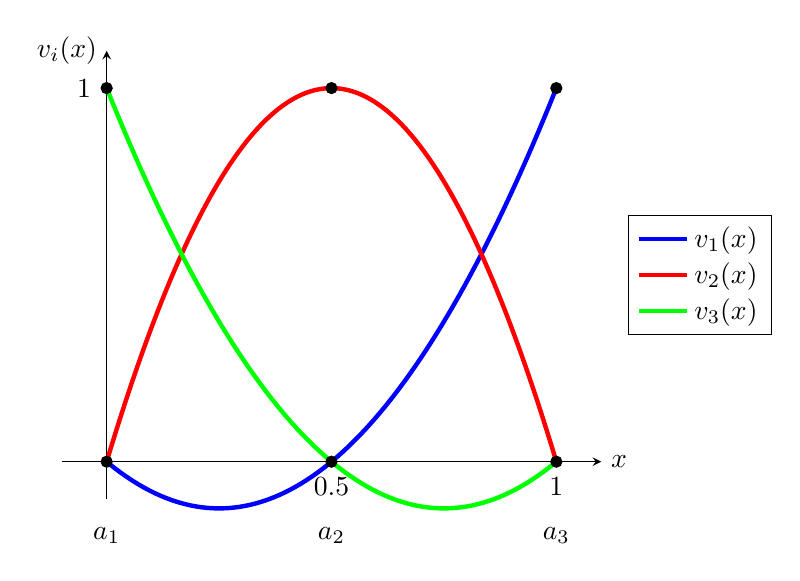
\begin{tikzpicture}
  \begin{axis}[
    axis lines = middle,
      xlabel = $x$,
      ylabel = {$v_i(x)$},
      xmin = -0.1, xmax = 1.1,
      ymin = -0.1, ymax = 1.1,
      xtick = {0,0.5,1},
      ytick = {0,1},
      clip=false,
      % axis line style={},
      xlabel style={right},
      ylabel style={left},
      legend style={at={(1.05,0.5)}, anchor=west},
      ]
      
      \addplot[domain=0:1, samples=100, ultra thick, blue] {2*x*(x-0.5)};
      \addlegendentry{$v_1(x)$};
      
      \addplot[domain=0:1, samples=100, ultra thick, red] {-4*(x-1)*(x-0)};
      \addlegendentry{$v_2(x)$};
      % \node[red, above] at (axis cs:0.5,1) {$1$};
      
      \addplot[domain=0:1, samples=100, ultra thick, green] {2*(x-0.5)*(x-1)};
      \addlegendentry{$v_3(x)$};
      
      % Add 6 black dots at the nodes in y = 0 and y = 1
      \addplot[only marks, mark=*] coordinates {(0,0) (0.5,0) (1,0)};
      \addplot[only marks, mark=*] coordinates {(0,1) (0.5,1) (1,1)};

      % Below the x-axis, write $a_1$, $a_2$, $a_3$ at the corresponding x-coordinates
      \node[below] at (axis cs:0,-.15) {$a_1$};
      \node[below] at (axis cs:0.5,-.15) {$a_2$};
      \node[below] at (axis cs:1,-.15) {$a_3$};
      
  \end{axis}
\end{tikzpicture}
\caption{Lagrangian basis functions $v_i$ for $k=2$ on the interval $[0,1]$ in dimension one. In this example, the choice of the support points is $a_1=0$, $a_2=0.5$, and $a_3=1$. The basis functions are quadratic and continuous, with each function equal to one at its corresponding support point and zero at the others.}
\label{fig:lagrange_basis}
\end{figure}

\subsection{Polynomial spaces on simplices and hypercubes}

For Lagrangian finite elements in dimensions two and three, we typically work with two types of polynomial spaces:

\begin{itemize}
\item $\mathbb{P}^k$ - the space of polynomials of total degree at most $k$ (used on simplices)
\item $\mathbb{Q}^k$ - the space of tensor-product polynomials with degree at most $k$ in each variable (used on quadrilaterals and hexahedra)
\end{itemize}

\subsubsection{Dimension of polynomial spaces}

For a $d$-dimensional domain:

\begin{itemize}
\item The dimension of $\mathbb{P}^k$ is $\binom{k+d}{d} = \frac{(k+d)!}{k!d!}$
\item The dimension of $\mathbb{Q}^k$ is $(k+1)^d$
\end{itemize}

In particular, for common cases:

\begin{table}[h]
\centering
\begin{tabular}{|c|c|c|c|}
\hline
\textbf{Space} & \textbf{1D} & \textbf{2D} & \textbf{3D} \\
\hline
$\mathbb{P}^1$ & $2$ & $3$ & $4$ \\
$\mathbb{P}^2$ & $3$ & $6$ & $10$ \\
$\mathbb{P}^3$ & $4$ & $10$ & $20$ \\
\hline
$\mathbb{Q}^1$ & $2$ & $4$ & $8$ \\
$\mathbb{Q}^2$ & $3$ & $9$ & $27$ \\
$\mathbb{Q}^3$ & $4$ & $16$ & $64$ \\
\hline
\end{tabular}
\caption{Dimensions of polynomial spaces $\mathbb{P}^k$ and $\mathbb{Q}^k$ in different dimensions}
\end{table}

\subsection{Selection of support points}

For Lagrangian elements, the selection of support points (nodes) is critical. The number of nodes must match the dimension of the polynomial space, and their placement must ensure unisolvence - that is, there must be a unique polynomial in the space that takes prescribed values at those nodes. Ensuring that there are enough nodes to span the polynomial space is necessary but not sufficient for the finite element to be unisolvant. As an example, consider any choice of three collinear nodes on a triangle. Such a choice is not unisolvent for the space $\mathbb{P}^1$, since in general we cannot choose the values of a linear polynomial at these three points independently, and when a linear polynomial exists, it is not unique. To generate a unique linear polynomial, we need to choose three non-collinear points. Any collection of three non-collinear points in $\R^2$ is unisolvent for the space of linear polynomials.

\subsubsection{Unisolvent sets of points}

For a set of points $\{x_i\}_{i=1}^n$ to be unisolvent for a polynomial space $P$ of dimension $n$, the only polynomial in $P$ that vanishes at all these points must be the zero polynomial. Equivalently, the interpolation problem: find $p \in P$ such that $p(x_i) = y_i$ for given values $\{y_i\}_{i=1}^n$ must have a unique solution.

\subsubsection{Simplicial elements}

For simplicial elements (triangles in 2D, tetrahedra in 3D) using $\mathbb{P}^k$, common choices include:

\begin{itemize}
\item $\mathbb{P}^1$: Vertices of the simplex
\item $\mathbb{P}^2$: Vertices and midpoints of edges
\item $\mathbb{P}^3$: Vertices, points dividing each edge into three equal parts, and one interior point (see Figure~\ref{fig:p_nodes_2d})
\end{itemize}

\begin{figure}[!htb]
\centering
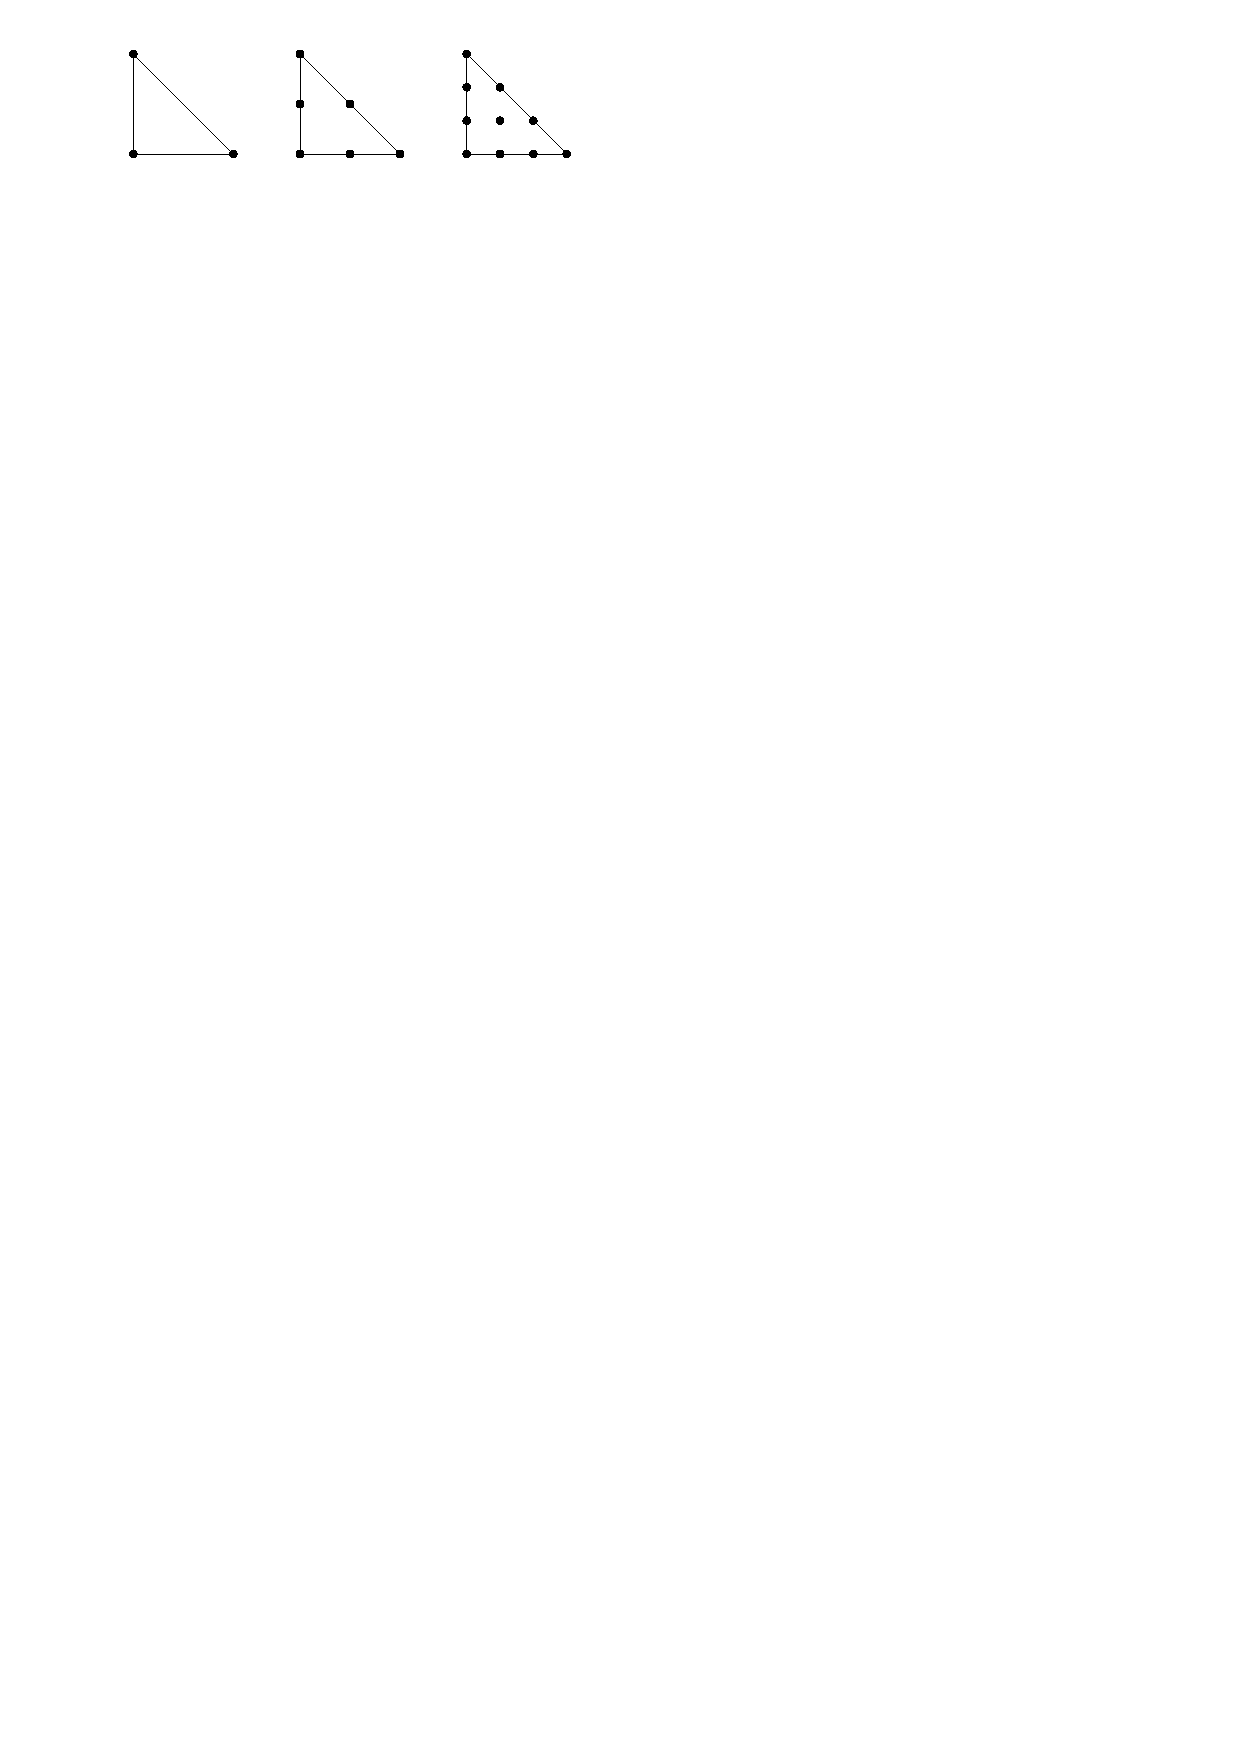
\includegraphics{lagrange_nodal_functions_triangles.pdf}
\caption{Position of nodes for $\mathbb{P}^1, \mathbb{P}^2$, and $\mathbb{P}^3$ on a triangle.}
\label{fig:p_nodes_2d}
\end{figure}

\subsubsection{Quadrilateral and hexahedral elements}

For quadrilateral elements in 2D and hexahedral elements in 3D using $\mathbb{Q}^k$, nodes are typically placed at:

\begin{itemize}
\item $\mathbb{Q}^1$: Vertices of the hypercube
\item $\mathbb{Q}^2$: Vertices, midpoints of edges, and (in 2D) the center of the quadrilateral
\end{itemize}

More generally, for $\mathbb{Q}^k$ on a hypercube, nodes are often placed as tensor products of 1D Lagrange interpolation points (see Figure~\ref{fig:q_nodes_2d}).


\begin{figure}[!htb]
  \centering
  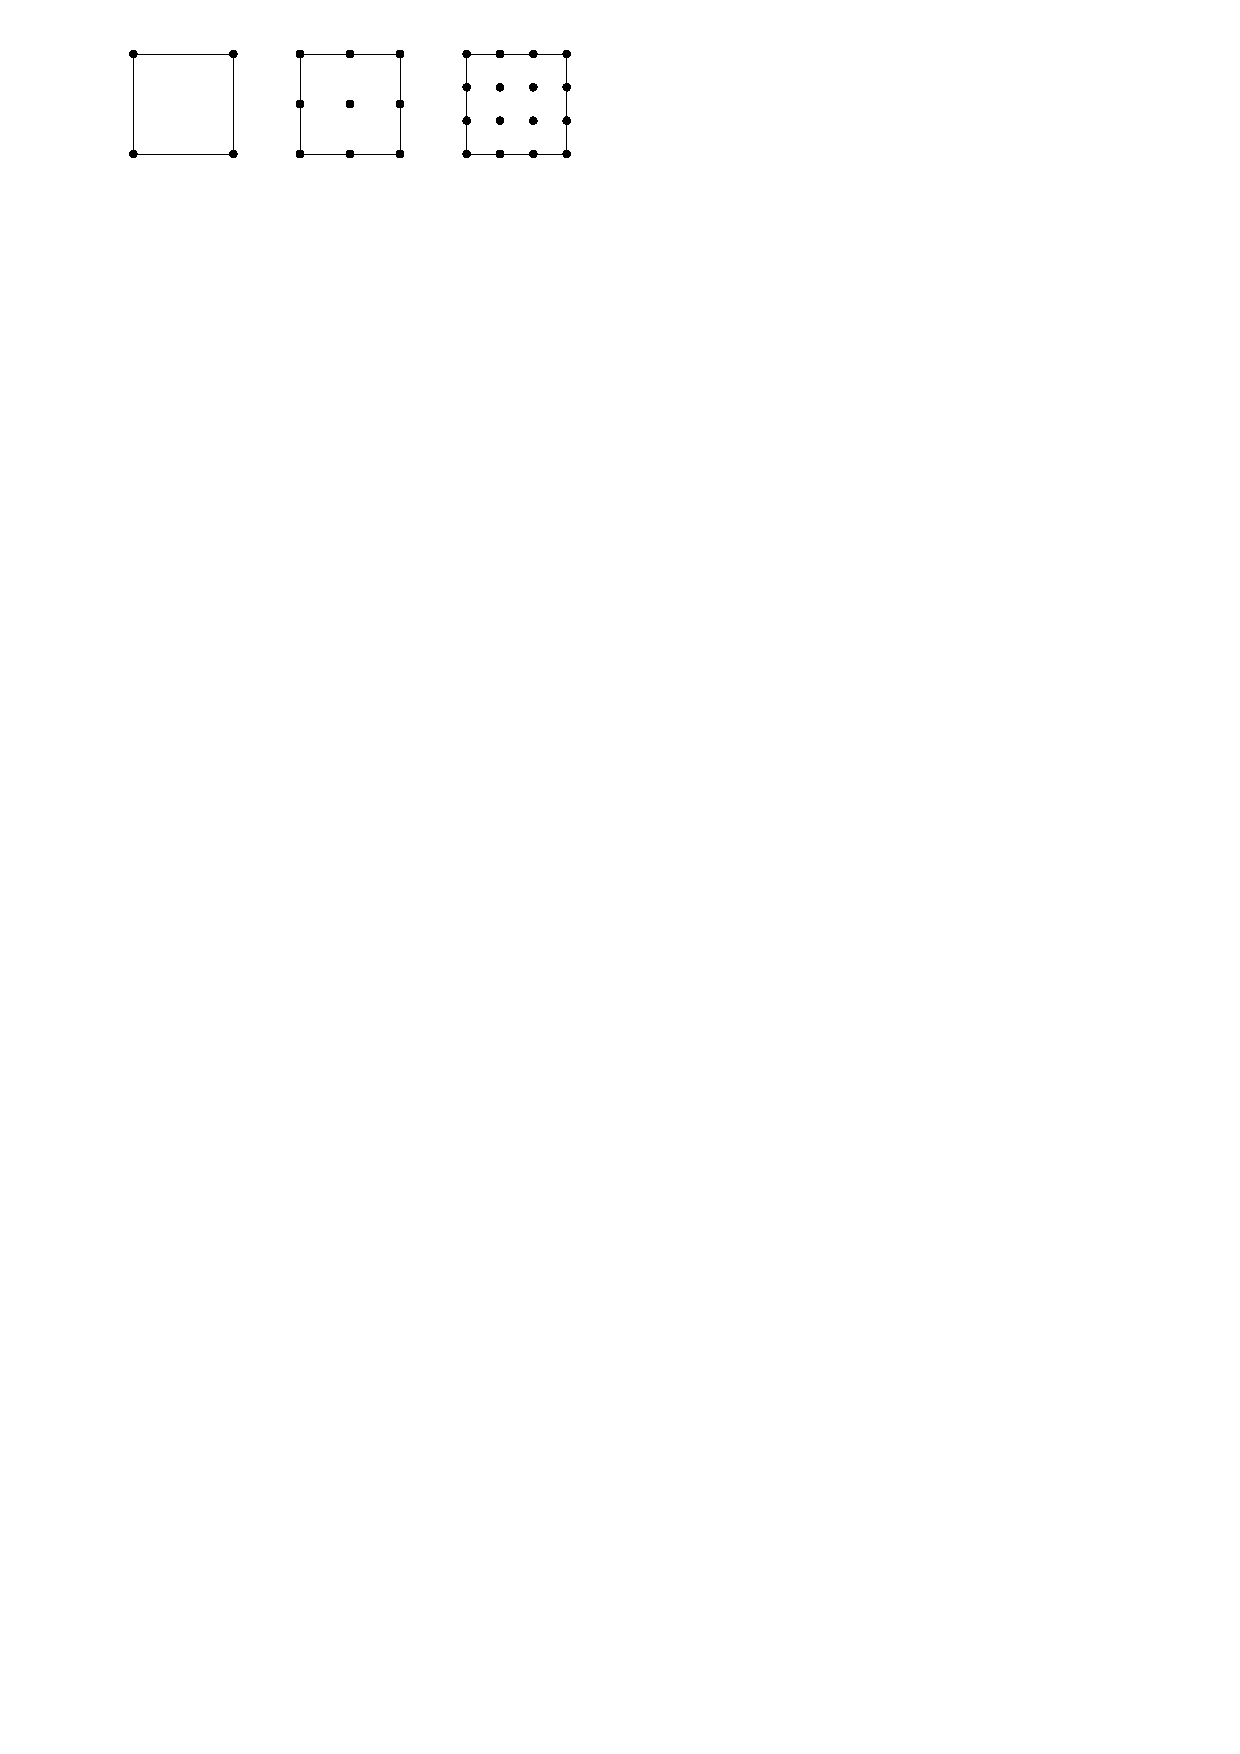
\includegraphics{lagrange_nodal_functions_quads.pdf}
  \caption{Position of nodes for $\mathbb{Q}^1$, $\mathbb{Q}^2$, and $\mathbb{Q}^3$ on a square.}
  \label{fig:q_nodes_2d}
  \end{figure}

\subsection{Polynomial conformity}

A critical property for polynomial based finite element spaces is that the restriction of the polynomial space on any lower-dimensional entity (i.e., face, edge, or point) is a polynomial space of the same degree on that lower-dimensional entity. The dimension of the polynomial space on the lower-dimensional entity follows from the polynomial degree and the dimension of the entity.

\begin{definition}[Polynomial conformity] \marginpar{Polynomial conformity}
Let $T$ be a $d$-dimensional element (e.g., a line, triangle, quadrilateral, tetrahedron, or hexahedron) and let $\mathbb{X}^i$ be an $i$-dimensional entity of $T$ (i.e., one of its faces, edges, or vertices). A Lagrange finite element space is said to be polynomially conforming of degree $k$, if the number of support points located on each $i$-dimensional entity $\mathbb{X}^i$ (including all its lower dimensional entities) is equal to the dimension of the polynomial space on that entity, with the convention that the dimension of the polynomial space on a $0$-dimensional entity (i.e., a vertex) is $1$ for $k \geq 1$ and $0$ for $k=0$.
\label{def:polynomial_conformity}
\end{definition}

\begin{figure}
\centering
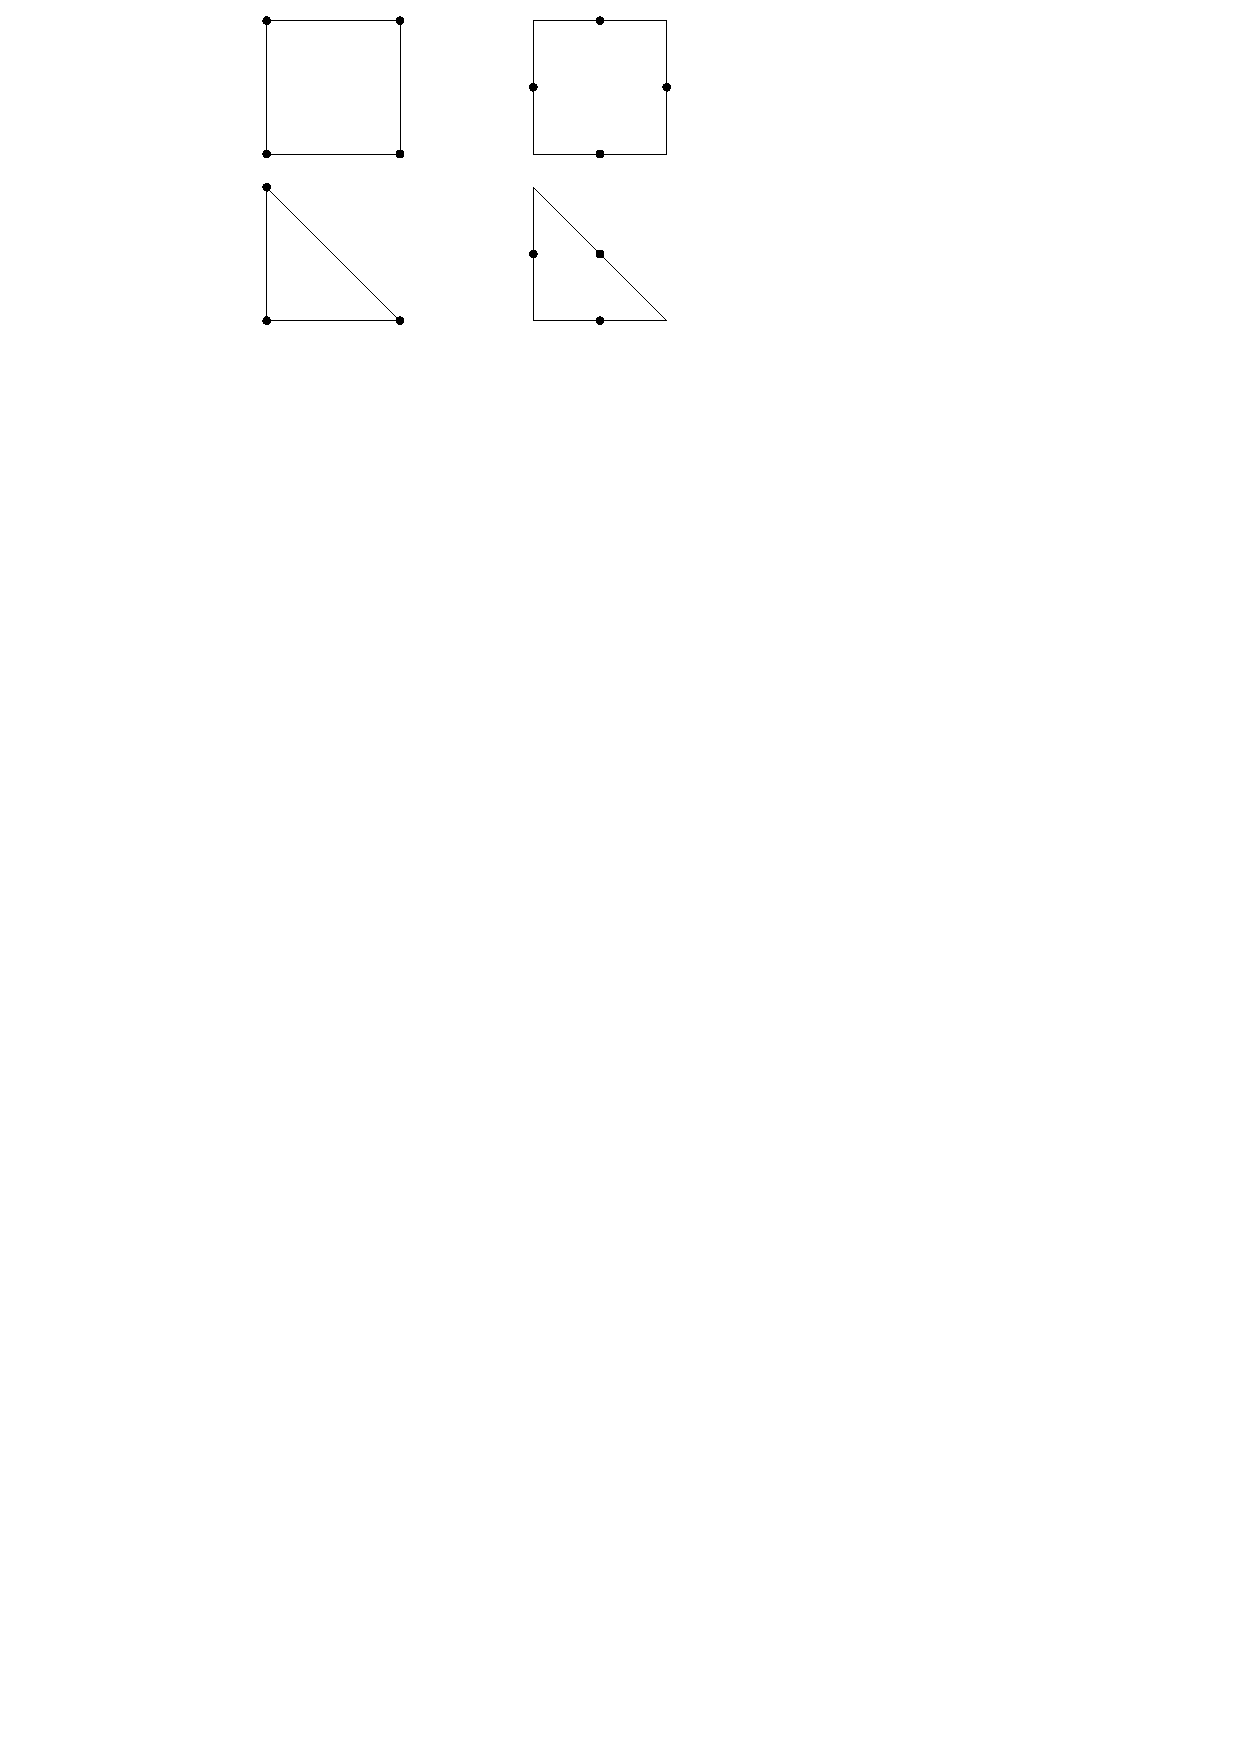
\includegraphics[width=.7\textwidth]{polynomial_conformity.pdf}
\caption{Polynomial conformity: the number of nodes on any any lower-dimensional entity (i.e., face, edge, or point) must match the dimension of the restriction of the polynomial space on that lower-dimensional entity. On the left we see polynomially conforming quadrilateral and triangular elements of degree $k=1$, where the number of nodes on the edges (two) matches the dimension of the polynomial space on the edges. On the right, we see non-polynomially conforming elements (namelly the Crouzier-Raviart elements), where the number of nodes on the edges (one) does not match the dimension of the polynomial degree of the restriction.}
\label{fig:polynomial_conformity}
\end{figure}

Considering, for example, the case of a $\mathbb{P}^3$ finite element on a triangle (see Figure~\ref{fig:p_nodes_2d} -- right), we have the following:
\begin{itemize}
\item The triangle has $3$ vertices, $3$ edges, and $1$ face.
\item The polynomial space $\mathbb{P}^3$ on the triangle has dimension $10$.
\item The polynomial space $\mathbb{P}^3$ on each edge has dimension $4$.
\item The polynomial space $\mathbb{P}^3$ on each vertex has dimension $1$.
\end{itemize}

Starting from the lower-dimensional entities, if we want to ensure polynomial conformity, we musth define, respectively:
\begin{itemize}
\item $1$ node on each vertex;
\item $2$ nodes on the interior of the edges (so that, including the vertices, we have $4$ nodes on each edge);
\item $1$ node on the interior of the triangle (so that, including the edges, we have a total of $10$ nodes on the triangle).
\end{itemize}

\begin{remark}
Polynomial conformity \emph{per-se} is not required to define a Lagrangian finite element (and it is in fact often not asked, see, for example, the definition of the Crouzier-Raviart elements in Figure~\ref{fig:polynomial_conformity}). It is however a necessary condition to ensure inter-element continuity, i.e., if we want to glue together different \emph{local} finite elements, and to ensure that the resulting \emph{global} finite element space is continuous.
\end{remark}

\subsection{Triangulations}

The definition of a global finite dimensional space is then constructed by
glueing together many small local finite element spaces. This is achieved
through the concept of \emph{triangulation} of the domain $\Omega$. The idea is
to partition the domain $\Omega$ into simple subdomains (like triangles or
quadrilaterals in 2D and tetrahedra, hexahedra, prisms, or pyramids in 3D) where
it is easy to define local basis functions, and to compute integrals. Once the domain is partitioned, we
define a finite dimensional space on each of these subdomains, and then ``glue them together'' to form a global finite dimensional space.

Formally speaking we partition $\Omega$
\begin{equation*}
\Omega = \mathring{\overline{\Bigl(\bigcup_{m=1}^M T_m \Bigr)}}
\end{equation*}
into a set of simple (closed, Lipschitz, and convex) subdomains $T_m$ (called \emph{elements} or \emph{cells})
such that 
\begin{equation}
T_i \cap T_j = \begin{cases}\emptyset \\ \text{vertex} \\ \text{common edge or face}.\end{cases}
\end{equation}
We call this partition a \emph{triangulation} $\mathcal{T}_h$, where
``triangulation'' is just an historical term, and we assume that we can have
triangulations composed of different shapes.

In what follows, we assume for simplicity that a triangulation is made by
elements or cells that are all of the same type (e.g. all triangles, all
quadrilaterals, etc.). In this case we say that the triangulation is
\emph{regular}.

Figure~\ref{fig:triangulation} shows an example of a triangulation of a two-dimensional domain. The domain is divided into a set of triangular elements, which are used to approximate the geometry and define finite element spaces.

The two tables below provide the minimal data structure required to describe this triangulation. The first table lists the coordinates of the vertices, while the second table specifies the connectivity of the triangles, i.e., which vertices form each triangle.

\begin{figure}[!htb]
\centering
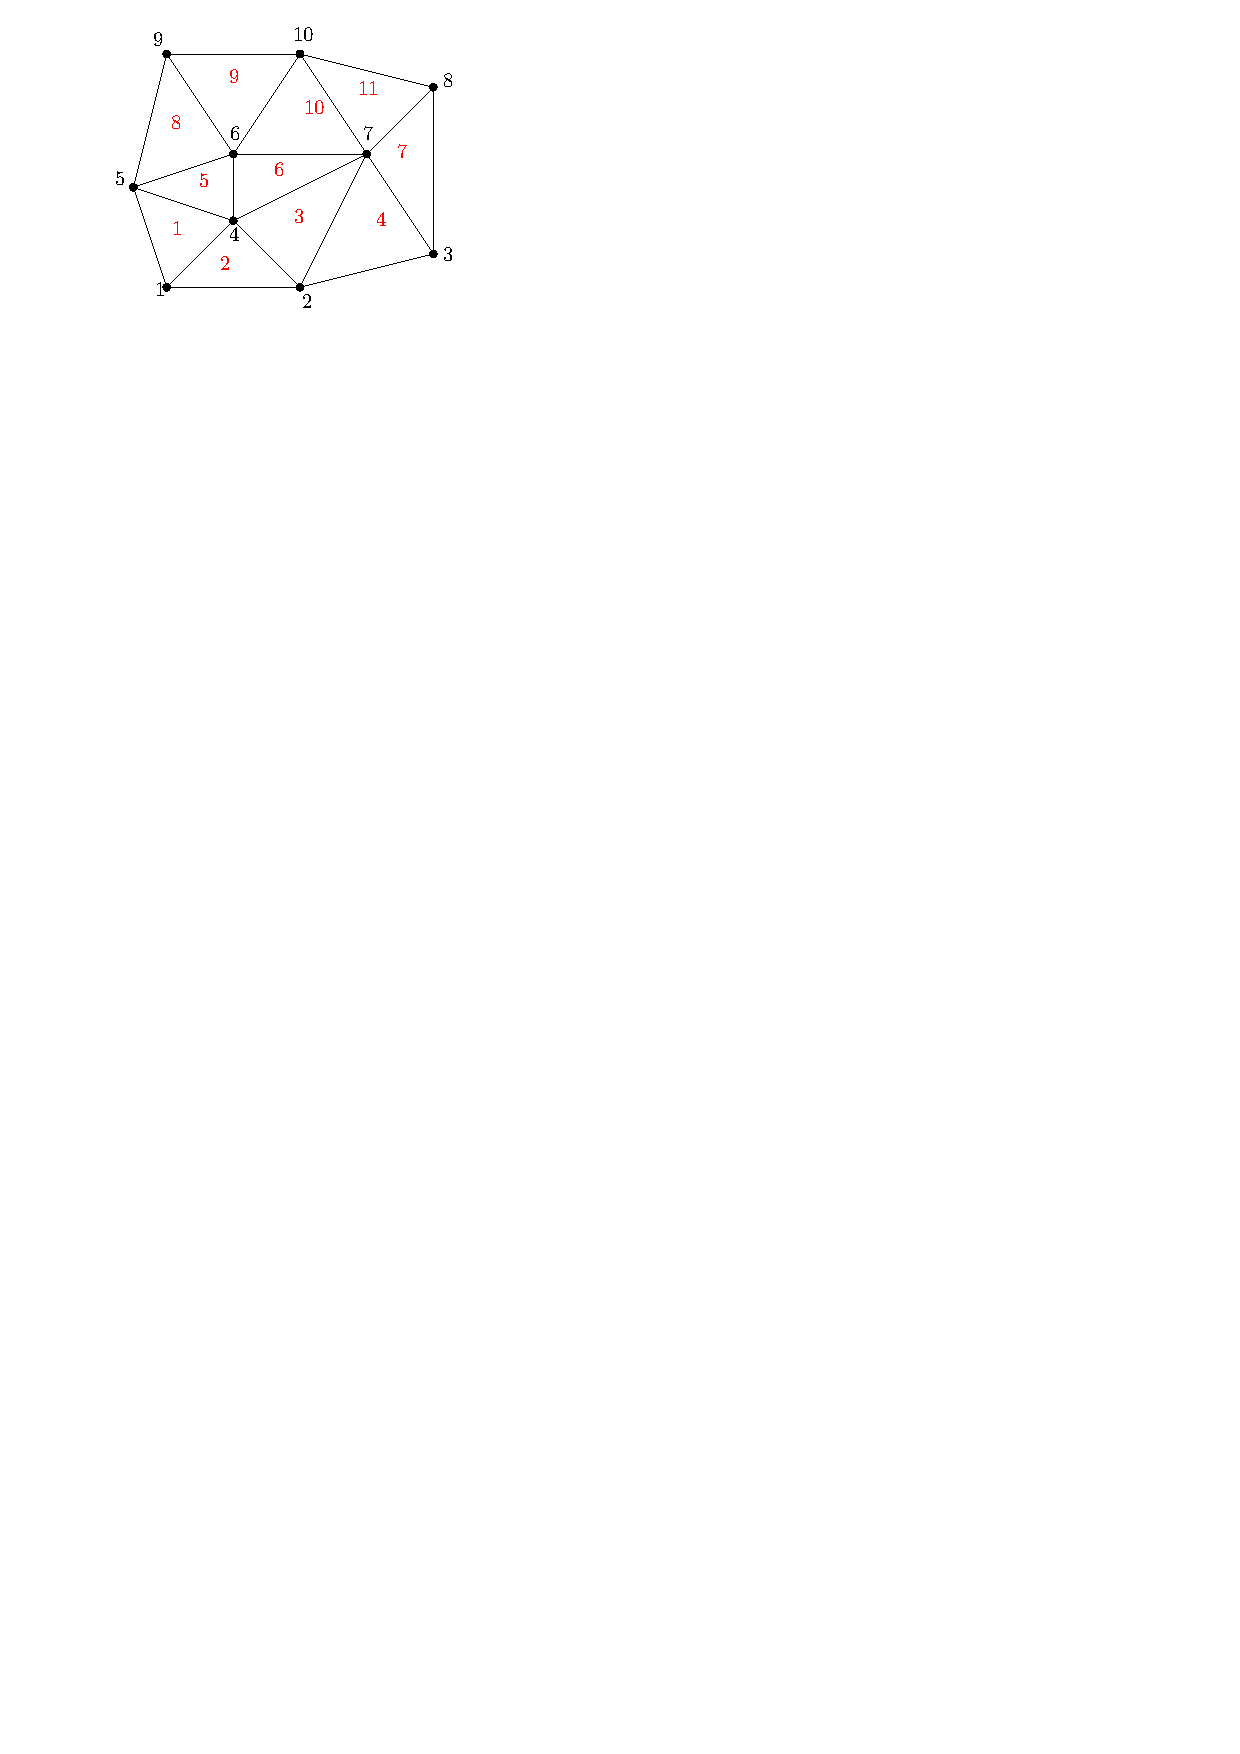
\includegraphics[width=.7\textwidth]{ball_2.pdf}
\caption{An example of a triangulation in $\R^2$. The domain is divided into triangular elements.}
\label{fig:triangulation}
\end{figure}

\begin{table}[!htb]
  \centering
  \caption{Miniimal data structure of a triangulation: a list of vertex coordinates (left), and a list of triangle connectivity (right).}
  \label{tab:vertex-coordinates}
  \begin{minipage}[t]{0.45\textwidth}
    \centering
  \begin{tabular}{|c|c|c|}
  \hline
  \textbf{Vertex} & $x_1$ & $x_2$ \\ \hline
  1 & 0.0 & 0.0 \\ \hline
  2 & 0.5 & 0.0 \\ \hline
  3 & 1.0 & 0.0 \\ \hline
  4 & 0.5 & 0.5 \\ \hline
  5 & 0.0 & 0.5 \\ \hline
  6 & 1.0 & 0.5 \\ \hline
  7 & 1.5 & 0.5 \\ \hline
  8 & 2.0 & 0.5 \\ \hline
  9 & 0.5 & 1.0 \\ \hline
  10 & 1.5 & 1.0 \\ \hline
  \end{tabular}
\end{minipage}
\begin{minipage}[t]{0.45\textwidth}
  \centering
  \begin{tabular}{|c|c|c|c|}
    \hline
    \textbf{Triangle} & $v_1$ & $v_2$ & $v_3$ \\ \hline
    1 & 1 & 4 &  5 \\ \hline
    2 & 1 & 2 &  4  \\ \hline
    3 & 2 & 7 &  4 \\ \hline
    4 & 2 & 3 &  7 \\ \hline
    5 & 4 & 6 &  5 \\ \hline
    6 & 4 & 7 &  6 \\ \hline
    7 & 3 & 8 &  7 \\ \hline
    8 & 5 & 6 &  9 \\ \hline
    9 & 6 & 10 &  9  \\ \hline
    10 & 6 & 7 &  10 \\ \hline
    11 & 7 & 8 &  10 \\ \hline
    \end{tabular}
\end{minipage}
\end{table}

Implementing such data structure requires at the bare minimum two containers,
one for the vertex coordinates (generally stored as floating point numbers) and
one for the triangles (generally stored as a list of vertex indices, pointing to
entries in the first container). In general, it may be necessary also to store
(or to compute on the fly) additional information, such as edge connectivity
(i.e., which triangles share a common edge), vertex connectivty (i.e., which
triangles share a common vertex, or which edges share a common vertex), etc.
This information is useful for many purposes, such as mesh refinement, mesh
generation, and visualization. In practice, the data structure may be more
complex than the one shown in the example, depending on the specific
requirements of the application, but the basic idea remains the same: to store
the coordinates of the vertices and the connectivity of the elements in a way
that allows efficient access and manipulation of the mesh data.

\subsection{Enumeration of degrees of freedom}

Once we have defined a triangulation and chosen a finite element type, we need to decide how to distribute and enumerate the local degrees of freedom (DoFs) defined on each element of the mesh to global degrees of freedom. This process establishes a relationship between local DoFs on each element and their global indices in the resulting finite dimensional space.

Generally speaking, given a finite dimensional space $V_h$ defined on the triangulation $\mathcal{T}_h$, we need a way to identify the DoFs of the global space $V_h$ with the local DoFs defined on each element $T_m \in \mathcal{T}_h$. This is done for both the shape functions $v_i$ and the nodal functions $v^i$. The process of assigning global indices to local DoFs is called \emph{enumeration}. Given a local finite element $(T_m, P_m, \Sigma_m)$ with dimension $N_m = \dim(P_m)$, the enumeration process consists in defining a relationship between $v_{m~\alpha}$ and $v_{i}$, where $v_{m~\alpha}$ are the local shape functions defined on the element $T_m$ and $v_{i}|_{T_m} = v_{m~\alpha}$ are the global shape functions defined on the global finite dimensional space $V_h$, i.e., 
\[
  v_{\mathcal{I}_{m\alpha}}(x) = v_{m~\alpha}(x) \quad x \in T_m, \qquad m = 1,\ldots,M, \quad \alpha = 1,\ldots,N_m.
\]

The index $i = \mathcal{I}_{m\alpha} \in [1,n \equiv\dim(V_h) ]$ is the global index of the local basis function $v_{m~\alpha}$, and it is often conveniently defined through the permutation matrix $P_{m~i\alpha}$ that maps the local index $\alpha$ to the global index $i$:
\[
  v_{i}(x) = \sum_{\alpha=1}^{N_m} P_{m~i\alpha} v_{m~\alpha}(x) \quad x \in T_m, \qquad m = 1,\ldots,M, \quad i = 1,\ldots,n.
\]
where 
\[
  P_{m~i\alpha} = \begin{cases}
    1 & \text{if } i = \mathcal{I}_{m\alpha}, \\
    0 & \text{otherwise}.
  \end{cases}
\]

The construction of the permutation matrix $P_{m~i\alpha}$ (or of the indexing function $\mathcal{I}_{m\alpha}$) is the key step in the enumeration process, and it defines both the global DoF numbering and the properties of the global finite element space.

\subsubsection{Degrees of freedom per object}

A fundamental concept in DoF enumeration is the ``degrees of freedom per object'' vector ($\dpo$). This vector is attached to a finite element space and it specifies how many DoFs are \emph{logically} associated with each type of topological entity in the mesh:

\begin{itemize}
  \item $\dpo_0$: Number of DoFs per vertex
  \item $\dpo_1$: Number of DoFs per edge (excluding vertices)
  \item $\dpo_2$: Number of DoFs per surface (excluding edges and vertices)
  \item $\dpo_3$: Number of DoFs per volume (excluding surfaces, edges, and vertices)
\end{itemize}

Notice that the $\dpo$ vector is defined in a \emph{logical} sense, i.e., it does not necessarily depend on the actual position of the nodes on the mesh entities. The $\dpo$ vector is a property of the \emph{global} finite element space, rather than of the \emph{local} one,  and it is used to determine how many indices need to be assigned to each mesh entity during the enumeration process.

For example, the DoF distribution for common Lagrangian elements would be given by Table~\ref{tab:dof_distribution}.

\begin{table}[!h]
\centering
\begin{tabular}{|l|c|c|c|c|}
\hline
\textbf{Element} & $\dpo_0$ & $\dpo_1$ & $\dpo_2$ & $\dpo_3$ \\
\hline
$\mathbb{P}^1_0$ Triangle & 1 & 0 & 0 & 0 \\
$\mathbb{P}^2_0$ Triangle & 1 & 1 & 0 & 0 \\
$\mathbb{P}^3_0$ Triangle & 1 & 2 & 1 & 0 \\
$\mathbb{P}^1_{-1}$ Triangle & 0 & 0 & 3 & 0 \\
$\mathbb{P}^2_{-1}$ Triangle & 0 & 0 & 6 & 0 \\
$\mathbb{P}^3_{-1}$ Triangle & 0 & 0 & 10 & 0 \\
$\mathbb{P}^3_0$ Tetrahedra & 1 & 2 & 1 & 0 \\
$\mathbb{P}^4_0$ Tetrahedra & 1 & 3 & 3 & 1 \\
$\mathbb{P}^3_{-1}$ Tetrahedra & 0 & 0 & 0 & 20 \\
$\mathbb{P}^4_{-1}$ Tetrahedra & 0 & 0 & 0 & 35 \\
\hline
$\mathbb{Q}^1_0$ Quadrilateral & 1 & 0 & 0 & 0 \\
$\mathbb{Q}^2_0$ Quadrilateral & 1 & 1 & 1 & 0 \\
$\mathbb{Q}^2_0$ Hexahedra & 1 & 1 & 1 & 1 \\
$\mathbb{Q}^1_{-1}$ Quadrilateral & 0 & 0 & 4 & 0 \\
$\mathbb{Q}^2_{-1}$ Quadrilateral & 0 & 0 & 9 & 0 \\
$\mathbb{Q}^2_{-1}$ Hexahedra & 0 & 0 & 0 & 27 \\
\hline
\end{tabular}
\caption{DoF distribution per object for common element types. The first column indicates the type of element, while the other columns show the number of DoFs associated with vertices, edges, faces, and volumes, respectively. The subscript on the element type indicates the global continuity of the element, i.e., $\mathbb{P}^1_0$ is a globally continuous piecewise linear polynomial space, while $\mathbb{P}^1_{-1}$ is a discontinuous piecewise linear polynomial space.}
\label{tab:dof_distribution}
\end{table}

\begin{remark}[$\dpo$ and polynomial conformity]
  The $\dpo$ vector is closely related to the polynomial conformity property discussed earlier. For a finite element to be polynomially conforming, the number of DoFs assigned to each entity must match the dimension of the polynomial space on that entity. Notice however that there is a difference between the \emph{logical} association of DoFs to entities (i.e., the $\dpo$ vector) and the \emph{physical} association of DoFs to entities (i.e., the actual position of the nodes on the entities). For Lagrangian finite element spaces, the physical association of DoFs to entities is determined by the choice of support points and the polynomial degree. It is perfectly possible to have the same physical association for finite element spaces $\mathbb{P}^k_{0}$ and $\mathbb{P}^k_{-1}$, with a different logical association (i.e., a different global enumeration). For example, in the case of $\mathbb{P}^1_{0}$ and $\mathbb{P}^1_{-1}$ on a triangle, we have $\dpo_i = \delta_{1i}$ and $\dpo_i = 3\delta_{2i}$, respectively, but the physical location of the nodes could coincide (i.e., the $3$ nodes in the second case could be chosen to be physically on the vertices, even though they are not \emph{logically} assigned to vertices, i.e., $\dpo_0 = 0$ in the second case).
\end{remark}

\subsubsection{DoF enumeration algorithm}

To understand the consequences of different choices for the $\dpo$ vector, we consider the actual degrees of freedom enumeration process, which typically follows a hierarchical approach, assigning indices to mesh entities in order of increasing dimension. Assuming a triangulation made of simplices, we can enumerate the DoFs as follows:

\begin{enumerate}
  \item Assign DoF indices to vertices: $0, 1, \ldots, \dpo_0 \cdot |V| - 1$, where $|V|$ is the number of vertices
  \item Assign DoF indices to lines: $\dpo_0 \cdot |V|, \ldots, \dpo_0 \cdot |V| + \dpo_1 \cdot |L| - 1$, where $|L|$ is the number of lines
  \item Assign indices to triangles: $\dpo_0 \cdot |V| + \dpo_1 \cdot |L|, \ldots, \dpo_0 \cdot |V| + \dpo_1 \cdot |L| + \dpo_2 \cdot |T| - 1$, where $|T|$ is the number of triangles
  \item Assign indices to tetrahedra: $\dpo_0 \cdot |V| + \dpo_1 \cdot |L| + \dpo_2 \cdot |T|, \ldots, \dpo_0 \cdot |V| + \dpo_1 \cdot |L| + \dpo_2 \cdot |T| + \dpo_3 \cdot |Tets| - 1$, where $|Tets|$ is the number of tetrahedra.
\end{enumerate}

The total number of DoFs in the system is then:
\[
N_{dof} = \dpo_0 \cdot |V| + \dpo_1 \cdot |L| + \dpo_2 \cdot |T| + \dpo_3 \cdot |Tets|
\]

\subsubsection{Local-to-global DoF mapping}

We are now in the position to define the mapping $i=\mathcal{I}_{m~\alpha}$ (or the permuation matrices $P_{m~i\alpha}$) between local DoF indices $\alpha \in [1,N_m]$ of the element $T_m$ and the global indices $i \in [1, n]$. This mapping determines the relation between the local enumeration of DoFs and the global one and it is constructed during DoF enumeration by:

\begin{enumerate}
  \item Identifying all the topological entities of the element $T_m$ (vertices, edges, etc.)
  \item Looking up the global indices already assigned to those entities
  \item Creating an ordered list that maps each local DoF to its corresponding global index
\end{enumerate}

\subsubsection{Example}

Consider a simple triangulation with two triangles and $\mathbb{P}^2$ elements ($\dpo_0 = 1, \dpo_1 = 1, \dpo_2 = \dpo_3 = 0$):

\begin{figure}[h]
\centering
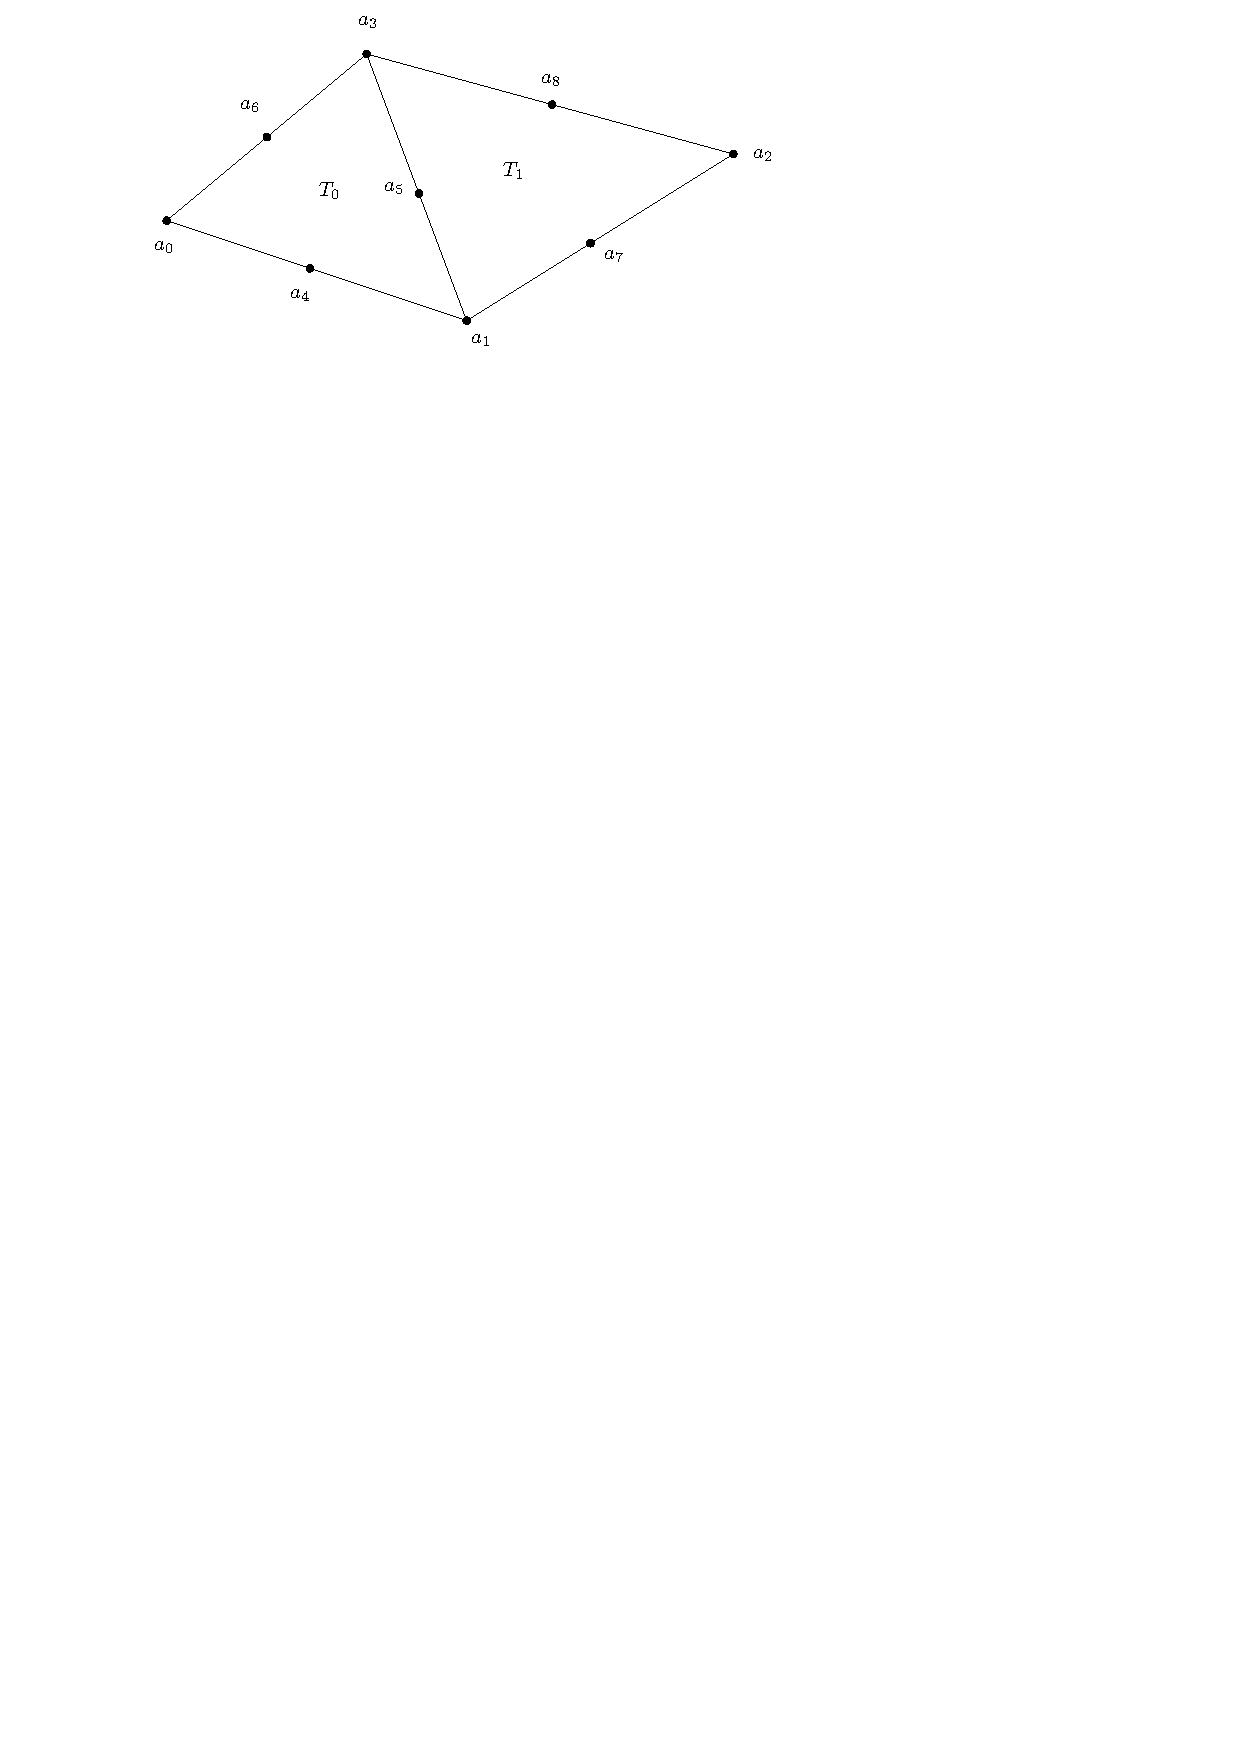
\includegraphics{dpo_example.pdf}
\caption{Simple triangulation with global vertex indices}
\end{figure}

The DoF mapping for these elements would be:
\begin{itemize}
  \item Element $T_1$: $\mathcal{I}_1 = [0, 1, 3, 4, 5, 6]$
  \item Element $T_2$: $\mathcal{I}_2 = [1, 2, 3, 7, 8, 5]$
\end{itemize}

This mapping ensures that the support points associated to the shared vertices and to the shared edge between elements are assigned the same global indices. Such a choice ensures global continuity of the finite element space, i.e., the finite element space is continuous across the entire triangulation. In particular, it holds:

\begin{theorem}[Continuity of Lagrange finite element spaces]
\label{thm:continuity_lagrange}
  Let $\mathcal{T}_h$ be a triangulation of the domain $\Omega$ and let $V_h$ be the finite element space defined on $\mathcal{T}_h$ using Lagrangian finite elements. Then, the finite element space $V_h$ is continuous across the entire triangulation if and only if the following conditions are satisfied:
  \begin{itemize}
    \item The support points satisfy the polynomial conformity property (Definition~\ref{def:polynomial_conformity});
    \item The $\dpo$ vector is defined such that also the \emph{logical} association between dofs and entities satisfies the polynomial conformity property (Definition~\ref{def:polynomial_conformity}), i.e., the sum of the number of DoFs assigned to each entity (vertex, edge, face, volume) must match the dimension of the polynomial space on that entity;
    \item The support points associated to shared entities must coincide.
  \end{itemize}
\end{theorem}
\begin{proof}
  The proof of this theorem follows from the definition of polynomial conformity (Definition~\ref{def:polynomial_conformity}) and the properties of Lagrangian finite elements. 
  
  We start by showing that the polynomial conformity property is necessary for continuity.
  
  Let $\Xi$ be the entity shared by two elements $T_i$ and $T_j$, i.e., 
  \[
  \Xi := T_i \cap T_j \subset \partial T_i \cap \partial T_j,
  \]
  and let $v^{i\alpha}$ and $v^{j\beta}$, with $\alpha \in [1,\hat{n}]$ be the nodal functions associated with  $\Xi$ for a Lagrange space of order $k$. The polynomial conformity property ensures that the number of DoFs assigned to $\Xi$ matches the dimension of the polynomial space on that entity, i.e., $ \hat{n} = \dim(P^k(\Xi))$. By taking a continuous function $u\in V\cap C^0(\overline{\Omega})$, we have that $\Pi^i(u)$ and  $\Pi^j(u)$ are both functions in $P^k(\Xi)$. Since the support points on $\Xi$ coincide for both $\Pi^i$ and $\Pi^j$, and their number is equal to the dimension of $P^k(\Xi)$, we conclude that  $\Pi^i(u) = \Pi^j(u)$ on $\Xi$. 
  
  Conversely, if we take two finite element functions $u_{h,i}$ and $u_{h,j}$ defined on the elements $T^i$ and $T^j$, there is no reasons why they should coincide on $\Xi$, unless their values on the coinciding support points $a_{i~\alpha}$ and $a_{j~\beta}$ coincide. In order for this to be true, there cannot be two \emph{different} values of $u$ associated to the two local indices $\alpha$ and $\beta$: the global index of two coinciding support points $a_{i~\alpha}$ and $a_{j~\alpha}$ must be the same.
  
  By the enumeration algorithm described above, this is true only if the entries of the $\dpo$ vector are consistent with the polynomial conformity property. In this case, every dof associated to a vertex, edge, face, or volume is assigned a unique global index, and the number of DoFs assigned to each entity (vertex, edge, face, volume) matches the dimension of the polynomial space on that entity. In particular, if the $\dpo$ vector is defined such that the logical association between DoFs on a shared entity $\Xi$ is consistent with the polynomial conformity property, then the global indices of the support points on $\Xi$ are the same for both elements $T_i$ and $T_j$, and therefore the values of the nodal functions associated to the shared entity $\Xi$ coincide, i.e., for any $\alpha$ there exists a $\beta$ such that $\mathcal{I}^{i~\alpha} = \mathcal{I}^{j~\beta}$, and therefore $v^{i\alpha}(u_{h,i}) = v^{j\beta}(u_{h,j})$ on $\Xi$, and we conclude that $u_{h,i} = u_{h,j}$ on $\Xi$.
\end{proof}

An illustration of this property is shown in Figure~\ref{fig:cg_vs_dg}, where we compare the numbering for a discontinuous and for a continuous Lagrangian finite element method of order two on two neighboring triangles.

\begin{figure}[!htb]
\centering
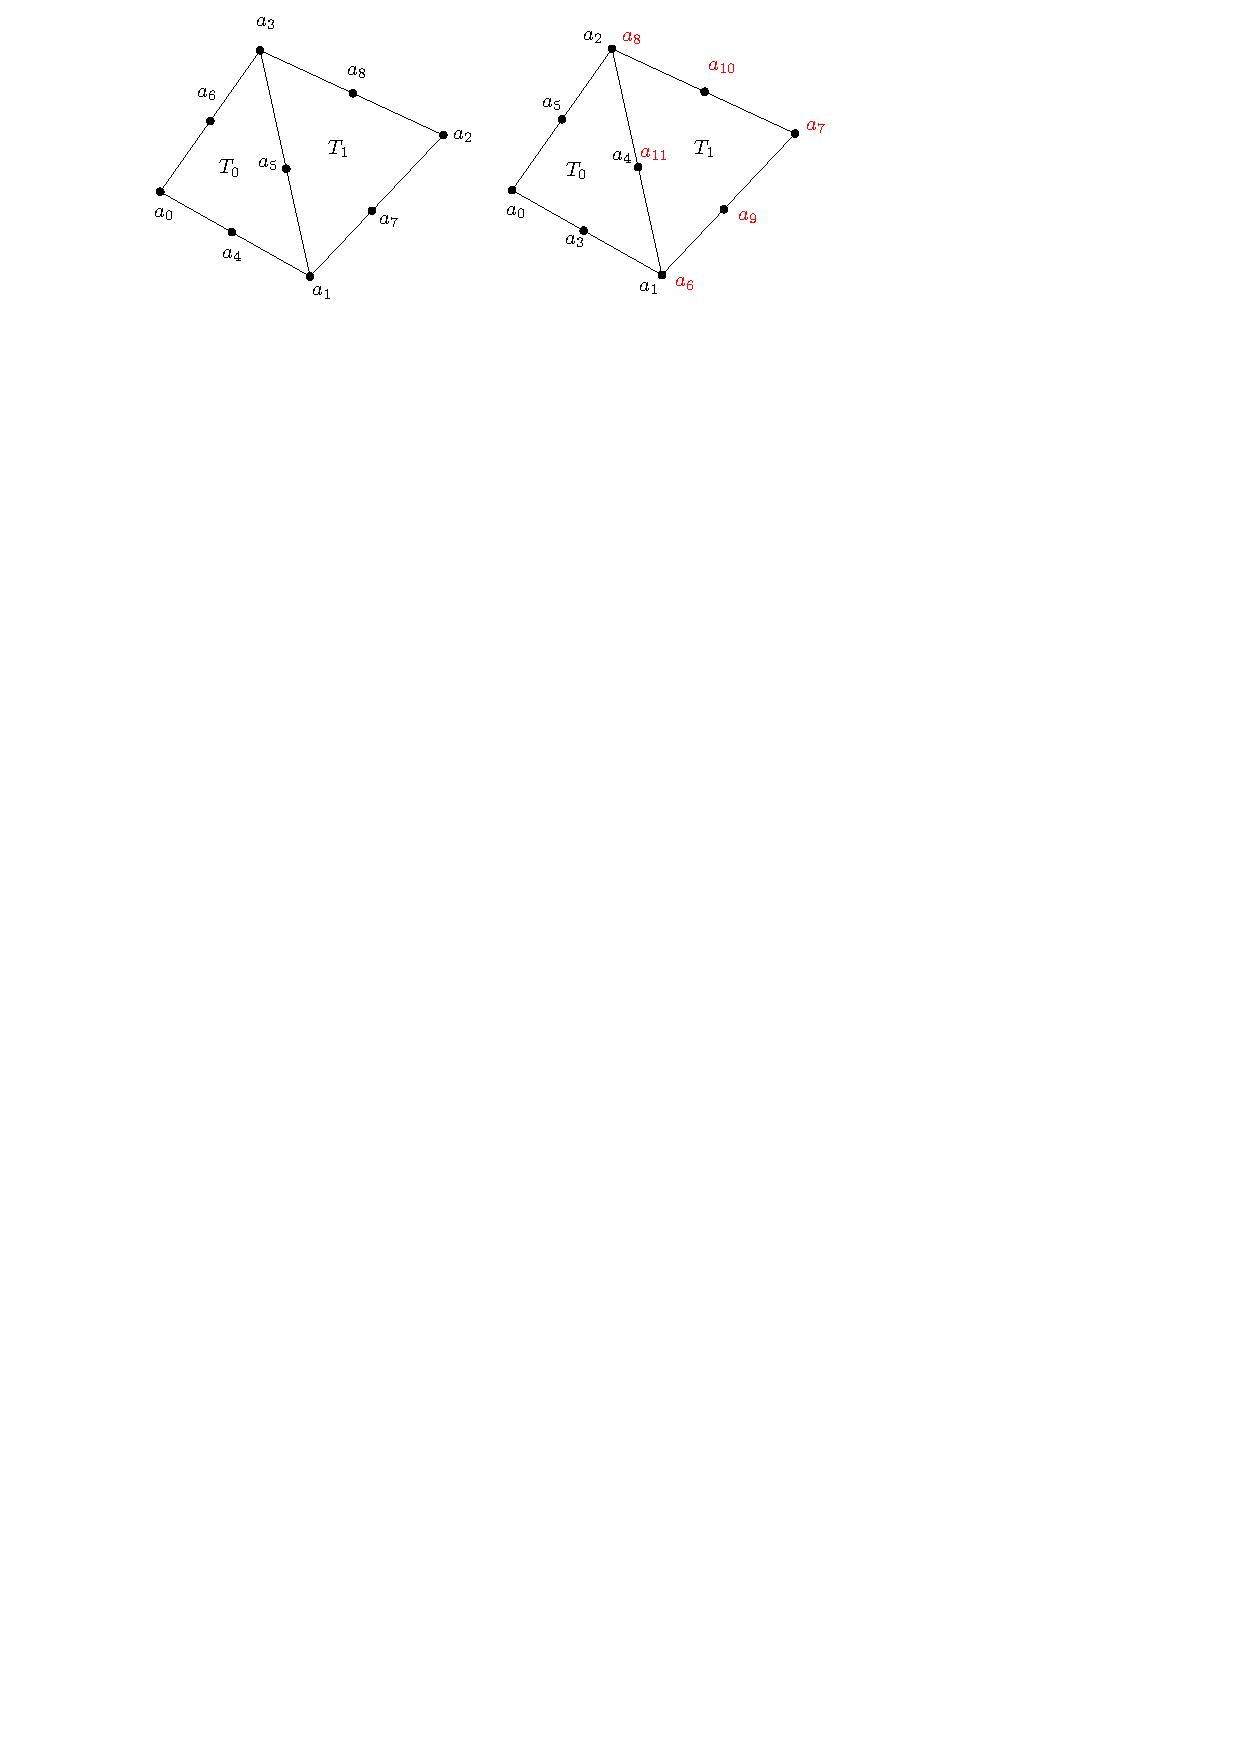
\includegraphics[width=.7\textwidth]{cg_vs_dg.pdf}
\caption{Comparison of the numbering for a continuous and for a discontinuous Lagrangian finite element method of order two on two neighboring triangles. Both finite element are polynomially conforming, and the support point locations coincide. The $\dpo$ vector on left is $\dpo = (1, 1, 0)$, while the $\dpo$ vector on the right is $\dpo = (0, 0, 6)$. We show the global indices of the support points on the left and on the right. The global indices of the support points on the shared edge are different for the discontinuous case, and we show in red the numbering in element $T_1$ for the discontinuous case.}
\label{fig:cg_vs_dg}
\end{figure}

For these two finite element spaces, we a global dimension $N_{cg} = 9$ on the left and $N_{dg} = 12$ on the right. The global indices of the support points on the shared edge are different for the discontinuous case, and we show in red the global numbering for the discontinuous case. In particular, in the discontinuous case, a discrete function is allowed to have different values in the points $(a_2, a_8)$, $(a_4, a_{11})$ and $(a_1, a_6)$. In the continuous case, those pairs of degrees of freedom are identified, and are associated with a single value of the discrete function (respectively, the entries with indices $3,5$ and $1$).

\begin{theorem}[Conformity of $V_h$ and $V$]
  For a global polinomial space $V_h$ to be conforming with the space $V \equiv W^{k,p}(\Omega)$, it is necessary and sufficient that the the space $V_h$ is continuous with degree of continuity $(k-1)$, i.e., $V_h \subset C^{k-1}(\overline{\Omega})$, with the understanding that $C^{-1}(\Omega)$ means that the space is discontinuous.
  
  In particular, a piecewise polynomial Lagrangian finite element space $V_h$ is continuous (therefore it is conforming w.r.t. $W^{1,p}(\Omega)$) if and only if i) the local finite element spaces are polynomially conforming, ii) the support points on shared entities coincide, and iii) their global indices are the same.
\end{theorem}